\documentclass[journal]{IEEEtran}
\IEEEoverridecommandlockouts
\usepackage{cite}
\usepackage{amsmath,amssymb,amsfonts}
\usepackage{algorithm}
\usepackage{algpseudocode}
\usepackage{graphicx}
\usepackage{textcomp}
\usepackage{booktabs}
\usepackage{array}
\usepackage{url}
\usepackage{multirow}
\usepackage[table]{xcolor}
% Make section/subsection headings stand out: IEEEtran's defaults (small-caps
% sections, italic subsections, all at normal size) are hard to tell apart.
\usepackage{titlesec}
\titleformat{\section}[block]
  {\centering\large\bfseries\scshape}{\thesection.}{0.6em}{}
\renewcommand{\thesubsection}{\Alph{subsection}}
\titleformat{\subsection}[block]
  {\bfseries\large}{\thesubsection.}{0.5em}{}
\titleformat{\subsubsection}[block]
  {\normalsize\bfseries\itshape}{\thesubsubsection)}{0.6em}{}
% Give headings clear vertical separation from the surrounding body text so the
% heading is visibly detached from the paragraph it introduces.
% {left}{above}{below}
\titlespacing*{\section}{0pt}{1.6ex plus .4ex minus .2ex}{1.0ex plus .2ex}
\titlespacing*{\subsection}{0pt}{1.5ex plus .3ex minus .2ex}{0.7ex plus .2ex}
\titlespacing*{\subsubsection}{0pt}{1.2ex plus .3ex minus .2ex}{0.5ex plus .2ex}
\def\BibTeX{{\rm B\kern-.05em{\sc i\kern-.025em b}\kern-.08em
    T\kern-.1667em\lower.7ex\hbox{E}\kern-.125emX}}

\begin{document}

\title{A Latch-On-Resistant, False-Alarm-Gated Lead-Time Metric for Bearing
Anomaly Detection --- and What It Reveals About SCADA-Rate Logging}

\author{Ansh~Goyal\\
\textit{Jaypee Institute of Information Technology, Noida, India}\\
Email: anshgoyal500@gmail.com}

\markboth{Manuscript -- Prognostics and Health Management}%
{Goyal: A False-Alarm-Gated Lead-Time Metric for Bearing Anomaly Detection}

\maketitle

\begin{abstract}
Anomaly detectors for rolling-element-bearing prognostics are usually judged by
classification accuracy, which answers \emph{whether} a fault is detected but not
\emph{how early}, nor at what false-alarm cost. We argue that the operationally
decisive quantity is \emph{lead time}---the warning interval before failure---and
we make it the primary object of evaluation through a \emph{latch-on--resistant,
false-alarm-gated} metric. Warning time is credited only when the false-alarm rate
over a data-anchored, leakage-free \emph{pre-onset} region is within a stated
budget $\tau$; we prove by construction (and by a released unit test) that a
degenerate ``latch-on'' detector, which would otherwise score maximal lead time,
is invalidated, while a detector that fires just after the true degradation onset
scores valid at zero false-alarm rate. A formal comparison against the Saxena
prognostic horizon shows the gate is decisive: on IMS the ungated horizon ranks
first exactly the detectors---Hotelling $T^2$, Isolation Forest, and EWMA---that
have \emph{no} valid operating point at a $10\%$ budget, whereas the gated metric
identifies the deployable choice (3$\sigma$), so the two rankings invert at the
top. We then apply the metric to a question of direct industrial relevance: does
the coarse, \emph{bin-averaged} logging of a SCADA historian destroy detection
lead time relative to simple decimation? Using nine detectors---four SPC charts
(3$\sigma$, EWMA, CUSUM, Hotelling $T^2$), Isolation Forest, three deep
reconstruction autoencoders (LSTM, TCN, Transformer), and an RMS-trend
baseline, with Deep SVDD additionally evaluated---under a controlled sweep that
holds window content and alarm persistence constant, we test this across four
inferential run-to-failure datasets: XJTU-SY ($n{=}10$), FEMTO/PRONOSTIA
($n{=}6$), University of Ferrara ($n{=}6$), and NASA IMS ($n{=}3$), with
bootstrap confidence intervals and run-level significance tests. The metric
correctly refuses to manufacture a positive effect. On the large multi-bearing
sets the aggregate-vs-decimate difference is null (median $|$diff$|$ at most eight
minutes, with Isolation Forest even \emph{reversing sign} on FEMTO); on IMS it
shows a \emph{consistent positive trend}---the same sign across all three runs for
every magnitude detector (3$\sigma$ median $+18.4$\,h; Isolation Forest
$+12.2$\,h; EWMA $+5.8$\,h; CUSUM $+5.4$\,h; Hotelling $T^2$ $+4.6$\,h)---but with
only $n{=}3$ independent runs this does not reach significance (exact sign test
floors at $p{=}0.25$) and does not survive multiple-comparison correction. Across
the $N{=}40$ detector$\times$dataset family \textbf{nothing survives Holm
correction} (smallest adjusted $p{=}1.00$). The defensible cross-dataset
conclusion is \textbf{non-destruction}: coarse SCADA-rate logging does not cost
bearing-fault warning time, and averaging is at worst neutral and may stabilize
the health signal. A real single-asset gas-turbine SCADA record
(aggregate-vs-decimate under a minute) is reported as a case study in the appendix
and excluded from the inferential family. We additionally validate a conformal
detector for distribution-free false-alarm control, present a
lead-time--vs--false-alarm trade-off analysis, and report feature-group and
spectral ablations showing that time-domain amplitude/impulsiveness statistics
carry the prognostic signal on IMS. The contribution is a metric that is
statistically honest by construction, together with a reproducible methodology and
an honest, counter-intuitive null result rather than a guaranteed positive effect.
\end{abstract}

\begin{IEEEkeywords}
Predictive maintenance, prognostics and health management, lead time, anomaly
detection, condition monitoring, rolling-element bearing, SCADA, conformal
prediction, statistical process control, remaining useful life.
\end{IEEEkeywords}

\IEEEpeerreviewmaketitle

\section{Introduction}

\IEEEPARstart{C}{ondition}-based maintenance (CBM) and prognostics and health
management (PHM) promise to replace fixed-interval servicing with data-driven
intervention, reducing both unplanned downtime and unnecessary maintenance
\cite{jardine2006,lee2014,lei2018}. Rolling-element bearings are the most
common failure mode in rotating machinery, and a large literature applies
statistical control charts, classical machine learning, and deep models to
detect incipient bearing faults from vibration \cite{randall2011,zhao2019}.
The economic case is well established: a warning delivered hours or days before
a catastrophic seizure lets an operator schedule an orderly shutdown, order
parts, and avoid secondary damage to shafts, housings, and couplings.

Despite this, most published detectors are evaluated with
\emph{classification} metrics---accuracy, precision/recall, ROC--AUC. These
answer ``was the failure detected?'' but not the question a maintenance planner
actually asks: \emph{``how many hours of warning did we get, and how often did
the system cry wolf?''} A detector that warns 48\,h ahead at a low
nuisance-alarm rate is operationally distinct from one that fires minutes
before breakdown or one that alarms every day. The prognostics community has
long advocated time-aware metrics \cite{saxena2008,saxena2010,goebel2011}, yet
lead time is rarely the headline quantity in detector benchmarks, and
\emph{ad hoc} lead-time definitions are easy to game. In particular, any
lead-time metric that does not pair warning time with a false-alarm constraint
can be trivially maximized by a detector that simply alarms from the first
sample---a ``latch-on'' exploit that earns the full run length as lead time
while being operationally useless.

A second, eminently practical question motivates this study. Industrial SCADA
historians rarely store raw high-rate vibration; they store \emph{decimated} or
\emph{time-averaged} summaries at a coarse logging interval
\cite{tautz2017}---seconds to minutes, rather than the tens of kilohertz at
which accelerometers are sampled. The folklore concern is that averaging
destroys the kurtosis and crest-factor transients that signal an incipient
spall: if true, the very act of long-term storage would blind any prognostic
algorithm that consumes the historian. Whether this is actually true is an
empirical question that, to our knowledge, has not been tested with a sound
lead-time metric across multiple datasets. The answer matters: if averaging is
harmless, operators can store compact, cheap, bin-averaged streams without
sacrificing warning time; if it is harmful, the implication is that
prognostics-grade monitoring requires separate high-rate acquisition.

This paper makes both questions precise and answers them. We state the arc
explicitly:

\textbf{Problem.} Detectors are ranked by classification accuracy, which ignores
\emph{how early} a warning arrives and \emph{at what false-alarm cost}; and it is
unknown whether the coarse, bin-averaged logging of a SCADA historian destroys
that warning time relative to plain decimation.

\textbf{Solution.} We make \emph{lead time gated by a leakage-free false-alarm
rate} the primary metric---warning time counts only when the pre-onset
false-alarm rate is within budget---so that the degenerate latch-on detector is
provably scored \emph{invalid} rather than winning.

\textbf{Method.} Under this metric we run a \emph{controlled} sampling sweep that
holds window content and alarm persistence constant, applied to \textbf{nine detectors} (four SPC charts, Isolation Forest, three
deep reconstruction autoencoders, and an RMS-trend baseline; Deep SVDD
additionally evaluated) across \textbf{four inferential run-to-failure
datasets}---XJTU-SY ($n{=}10$), FEMTO/PRONOSTIA ($n{=}6$), University of Ferrara
($n{=}6$), and NASA IMS ($n{=}3$), plus a real single-asset ONGC gas-turbine
SCADA record analyzed as a case study (Appendix~E)---with
\emph{run-level} significance tests (the run, not the within-run sampling factor,
is the unit of inference) and Holm correction.

\textbf{Finding.} The folklore is \textbf{refuted on every dataset tested}: historian-style
aggregation does \emph{not} destroy lead time. On the large multi-bearing sets
(XJTU-SY, FEMTO, Ferrara) the difference is negligible; on IMS it shows a
consistent positive \emph{trend} (not significant at $n{=}3$); the single-asset
turbine record agrees (case study, Appendix~E). The defensible cross-dataset
conclusion is \textbf{non-destruction}---decimation is never better, and averaging
is at worst neutral.

\textbf{Contributions.} We make five contributions.
\begin{enumerate}
\item A \emph{latch-on--resistant, false-alarm-gated, onset-relative lead-time
metric}. Warning time is credited only when the false-alarm rate over a
data-anchored, leakage-free pre-onset region is within a stated budget. We
prove---by construction and by a unit test that is part of the released code---that
a constant-on (latch-on) detector is scored invalid, while a detector that fires
just after the true degradation onset scores valid at zero false-alarm rate. We do
not claim the metric is unconditionally ungameable; we discuss residual gaming
surfaces in Section~\ref{sec:threats}.
\item A \emph{formal proof that gating changes the answer}. We give, to our
knowledge, the first formal comparison showing that an ungated prognostic-horizon
metric (the Saxena PH) produces a different and operationally misleading detector
recommendation relative to the false-alarm-budgeted metric
(Section~\ref{sec:saxena}, Tables~\ref{tab:latchon} and~\ref{tab:phrank}): on IMS
the detectors PH ranks first by raw lead---Hotelling $T^2$, Isolation Forest, and
EWMA---each have no valid operating point at a $10\%$ false-alarm budget, whereas
our metric correctly identifies 3$\sigma$ as the deployable choice.
\item A \emph{controlled SCADA-sampling methodology} that holds window content and
alarm persistence constant, so that any lead-time difference between the
historian's \emph{aggregate} mechanism and simple \emph{decimation} reflects
genuine information loss rather than a window-counting artifact of coarser time
grids.
\item A \emph{multi-dataset null result that is statistically honest by
construction}. Across XJTU-SY ($n{=}10$), FEMTO/PRONOSTIA ($n{=}6$), University of
Ferrara ($n{=}6$), and NASA IMS ($n{=}3$), with bootstrap confidence intervals and
run-level significance tests that treat the run---not the within-run sampling
factor---as the unit of inference, SCADA-rate aggregation does \emph{not} destroy
lead time---and on IMS shows a consistent positive trend for the
variance-sensitive control charts---while decimation is never better; nothing
survives Holm correction across the $N{=}40$ family.
\item \emph{Validation}: wiring and empirical validation of a conformal detector
for distribution-free false-alarm control, a lead-time--vs--false-alarm trade-off
analysis, feature-group and spectral ablations that localize the prognostic signal
to time-domain statistics on IMS, and a characterization of deep reconstruction
models (LSTM-AE, TCN-AE, Transformer-AD) showing they do not become competitive
with SPC charts within the tested training-fraction range $[0.20, 0.60]$ on
short-lived bearings; whether a crossover exists on long-runway assets remains
open (Section~\ref{sec:mindata}).
\end{enumerate}

\textbf{Scope of claims.} The empirical results are for rolling-element bearings
under approximately steady operating conditions; we make no claim of transfer to
gearboxes, blades, or variable-speed machinery. The sampling question is
specifically \emph{bin-averaged} historian storage versus \emph{decimated}
storage. The metric itself is failure-mode-agnostic: it applies wherever a
run-to-failure trajectory and a stationary normal region exist.

We deliberately report a result that is not the one we set out to find. Our
working hypothesis was that averaging would smear incipient-fault transients
and shorten lead time. It does not. We regard reporting the refutation, with
its dataset-dependent direction made explicit, as more valuable than a tidy but
unsupported positive claim.

\section{Related Work}

\subsection{Prognostics, CBM, and lead-time metrics}
Reviews of machinery diagnostics and prognostics
\cite{jardine2006,lei2018,lee2014} and of remaining-useful-life (RUL)
estimation \cite{si2011} establish the CBM/PHM framing in which a health
indicator is tracked and an alarm or RUL estimate is produced. Saxena
\emph{et al.} \cite{saxena2008,saxena2010} and Goebel \emph{et al.}
\cite{goebel2011} propose a family of prognostic-performance metrics---prognostic
horizon, $\alpha$--$\lambda$ accuracy, relative accuracy, and
\emph{timeliness}---that explicitly reward early, well-calibrated predictions.
Our onset-relative lead time is in this spirit: it measures warning time
relative to a degradation event rather than to an arbitrary positional marker.
We depart from prior practice in one key respect: we make the false-alarm
budget an integral part of the metric's validity condition rather than a
separately reported number, which is precisely what closes the latch-on
loophole. We further provide, to our knowledge, the first formal comparison showing
that an ungated prognostic-horizon metric produces a different and operationally
misleading detector ranking relative to a false-alarm-budgeted metric
(Section~\ref{sec:saxena}, Tables~\ref{tab:latchon} and~\ref{tab:phrank}). The
disagreement is not marginal: on IMS the detectors the prognostic horizon ranks
first by raw lead---Hotelling $T^2$, Isolation Forest, and EWMA---each have no valid
operating point at a $10\%$ false-alarm budget, while our metric correctly
identifies 3$\sigma$ as the deployable choice.

\subsection{Anomaly detectors and control charts}
Univariate and multivariate statistical-process-control charts---the
3$\sigma$ rule, the exponentially weighted moving average (EWMA)
\cite{roberts1959}, and Hotelling's $T^2$ \cite{hotelling1947}---remain
workhorses of industrial monitoring \cite{montgomery2009} because they are
interpretable and require little training data. In the unsupervised
machine-learning family, Isolation Forest \cite{liu2008} and the one-class SVM
\cite{scholkopf2001} are widely deployed; deep models such as LSTM
autoencoders \cite{hochreiter1997,malhotra2016,hundman2018} and Deep SVDD
\cite{ruff2018} have been applied to machine-health monitoring \cite{zhao2019}.
We evaluate representatives of both the classical and learning families under a
single, fixed hyperparameter protocol so that the comparison is about the
\emph{evaluation} and the \emph{sampling} question, not about detector tuning.

\textbf{Relation to published FEMTO/XJTU results.} The FEMTO/PRONOSTIA and XJTU-SY
campaigns are best known through the IEEE PHM~2012 challenge and subsequent
remaining-useful-life (RUL) studies \cite{nectoux2012,wang2020}, whose leading methods
report a \emph{RUL-error} score on the deliberately \emph{truncated} Test/Validation
copies of the bearings. Those numbers are not directly comparable to ours for two
structural reasons: (i) they estimate a continuous RUL on runs with \emph{no observed
failure}, whereas our metric measures early-warning lead time on the complete
run-to-failure trajectory and gates it on a pre-onset false-alarm budget; and (ii) they
do not report a false-alarm rate at all, so a method's RUL score says nothing about
whether its alarm would survive our $\tau$ gate---the very quantity we argue is
decisive. We therefore do not tabulate their RUL scores against our lead times, which
would be a category error. The classic \emph{normalized-RMS health-indicator with a
first-prediction-time threshold}---the workhorse baseline underlying most of that
literature---is represented here by our \texttt{rms\_trend} detector, evaluated under
the same gated metric as every other method; re-evaluating specific published
architectures under the gated metric (which requires their original code) is left as
future work.

\subsection{Uncertainty quantification and conformal prediction}
Conformal prediction \cite{vovk2005,laxhammar2014} provides a distribution-free
guarantee that the false-alarm rate is bounded by a target $\alpha$ under
exchangeability. This is attractive for prognostics because it converts a
detector's raw score into an alarm with an interpretable, finite-sample
false-alarm guarantee. We wire conformal calibration into the lead-time
pipeline and, rather than assuming the guarantee, test it empirically across
runs---including a run where exchangeability provably fails because the
``normal'' region already contains degradation.

\subsection{Vibration features}
Bearing-defect frequencies, spectral kurtosis \cite{antoni2006}, and envelope
(demodulation) analysis \cite{randall2011} are the classical frequency-domain
tools for bearing diagnostics. We include FFT band energies,
spectral kurtosis, and Hilbert-envelope amplitudes at the bearing
characteristic frequencies, and we ablate them against pure time-domain
statistics to see which family actually carries prognostic lead time under our
gated metric.

\subsection{SCADA-based condition monitoring}
Tautz-Weinert and Watson \cite{tautz2017} review SCADA-data condition
monitoring and note explicitly that historian aggregation is a recognized but
\emph{under-quantified} concern: practitioners suspect that coarse averaging
hurts fault detection, but the magnitude of the effect has not been measured
with a principled warning-time metric. The present paper addresses exactly this
gap, and reaches the perhaps surprising conclusion that, for bearing faults,
the concern is not borne out.

\section{Datasets}

We use four inferential run-to-failure datasets spanning controlled-lab and
cross-condition regimes, together with a single-asset real-historian case study
(Table~\ref{tab:datasets}). They were chosen so that the central sampling claim
is tested under genuinely different conditions: a high-rate raw-waveform rig
where aggregation can be simulated faithfully (IMS), two multi-bearing campaigns
(XJTU-SY and FEMTO/PRONOSTIA) that supply the statistical power a three-run rig
cannot, a second modern constant-condition rig (Ferrara), and---as a case study
only---a real historian stream that already \emph{is} SCADA-rate data (ONGC,
Appendix~E).

\textbf{IMS.} The NASA/IMS bearing dataset \cite{qiu2006} provides raw
20.48\,kHz accelerometer waveforms for three run-to-failure tests on a shaft
loaded with four bearings. Because the waveforms are raw, the aggregate/decimate
sweep can be applied faithfully at the signal level, and frequency-domain
features (spectral kurtosis, envelope) are meaningful. IMS test~3's failure label is set as documented in the released repository; the
justification appears in Appendix~C.

\textbf{XJTU-SY.} The XJTU-SY dataset \cite{wang2020} contributes ten
run-to-failure bearings under two operating conditions (five bearings each) at
25.6\,kHz, sampled in 1.28\,s snapshots once per minute. With $n{=}10$ it
provides the strongest generalization test in this study; its published
lifetimes range widely (52--533\,min), which deliberately stresses the metric
with both long-degrading and abrupt-failure bearings.

\textbf{FEMTO/PRONOSTIA.} The FEMTO/PRONOSTIA platform \cite{nectoux2012}
contributes a fourth, independent run-to-failure campaign: six Learning\_set
bearings under three operating conditions, with horizontal and vertical
accelerometers sampled in 0.1\,s snapshots at 25.6\,kHz once every 10\,s. We use
only the six Learning\_set bearings because they are run until the platform's
20\,g vibration stop---a failure, and hence a lead time, is actually
observed---whereas the Test\_set/Validation\_Set copies are deliberately
truncated mid-life for the IEEE PHM 2012 RUL-prediction challenge and would make
lead time undefined. Lifetimes span $\sim$1.4--7.8\,h. We deliberately
\emph{exclude} the Paderborn dataset \cite{lessmeier2016} from the lead-time
study: it comprises pre-damaged bearings measured at fixed operating conditions
for fault \emph{classification}, with no degradation timeline and no failure
event, so it cannot test a lead-time or sampling claim. Using it for the
headline would be a category error, and we say so rather than pad the dataset
count.

\textbf{University of Ferrara.} The University of Ferrara dataset \cite{arpa2024}
contributes a fifth, fully independent run-to-failure campaign: six self-aligning
double-row ball bearings under constant speed and radial load, with continuous
uniaxial vibration recorded at 25.6\,kHz throughout each bearing's entire lifecycle
(five-second snapshots, contiguous). Lifetimes span $0.7$--$6.8$\,h, similar to
FEMTO. Operating conditions are fixed, making the dataset directly compatible with
our onset detector without normalization; we use all six available runs (E1--E6).
The single accelerometer channel is duplicated into the two channel slots so the
channel-invariant feature schema applies unchanged. The dataset is included to
further test the non-destruction hypothesis with an independent 2024 rig; like FEMTO
and XJTU-SY, its short bearing lifetimes mean this campaign cannot confirm or deny
the IMS positive trend.

\begin{table}[t]
\caption{Datasets used in this study. ``Role'' indicates the function each
dataset plays in the argument. The four inferential datasets supply the run-level
statistics; ONGC is a single-asset case study (Appendix~E) and Paderborn is
excluded.}
\label{tab:datasets}
\centering
\footnotesize
\begin{tabular}{@{}llll@{}}
\toprule
Dataset & Role & Rate & Runs \\
\midrule
IMS \cite{qiu2006}      & controlled lab     & 20.48\,kHz raw    & 3 \\
ONGC                    & case study (App.~E) & 10\,s historian   & 1 \\
XJTU-SY \cite{wang2020} & generalization     & 25.6\,kHz, 1/min  & 10 \\
FEMTO \cite{nectoux2012}& generalization     & 25.6\,kHz, 1/10\,s& 6 \\
Ferrara \cite{arpa2024} & generalization     & 25.6\,kHz, continuous & 6 \\
Paderborn \cite{lessmeier2016} & excluded (no RUL) & 64\,kHz    & -- \\
\bottomrule
\end{tabular}
\end{table}

XJTU-SY ($n{=}10$) is our primary inferential dataset; IMS ($n{=}3$) is retained
for its raw-waveform access, which permits the faithful aggregate/decimate
simulation and the mechanism analysis (Appendix~D).

\section{Methodology}

\subsection{Problem formulation and notation}
For each run we observe a sequence of snapshots indexed by time $t$. A feature
extractor maps each snapshot (and a short trailing window) to a vector
$x_t \in \mathbb{R}^d$. A detector assigns a score $s_t$ and, via a threshold
and a persistence filter, an alarm indicator $a_t \in \{0,1\}$. Each run has a
failure time $t_f$ and is split at a train boundary $t_b$; all scaling and
threshold statistics are fit on $\{t \le t_b\}$ only. The two quantities we
care about are the \emph{lead time} (how long before $t_f$ the first sustained
alarm fires) and the \emph{pre-onset false-alarm rate} (how often the detector
alarms while the machine is still healthy). The remainder of this section makes
each ingredient precise.

\subsection{Channel-invariant feature schema}
Each snapshot yields per-channel time-domain statistics---RMS, kurtosis,
skewness, peak-to-peak, crest factor, and variance---and, for raw-waveform
datasets, frequency-domain features: FFT band energies, spectral kurtosis
\cite{antoni2006}, and Hilbert-envelope amplitudes at the bearing
characteristic frequencies (BPFO, BPFI, BSF, FTF), computed from the dataset
geometry.

A naive feature scheme that concatenates per-channel statistics and all
cross-channel pairs is \emph{channel-count dependent} and ill-posed: it produces
$445$ features for a 4-channel run and $1465$ for an 8-channel run, against only
$\sim$100 training snapshots, i.e.\ $p \gg n$. Such a space overfits, is not
comparable across runs with different channel counts, and silently inflates the
apparent dimensionality. We therefore aggregate each statistic family
\emph{across} physical channels (taking the mean and the max over channels) and
summarize each aggregated series over a rolling window with four descriptors
(mean, standard deviation, max, and linear-trend slope), plus one cross-channel
RMS-coherence feature. This yields a fixed $49$-dimensional space that is
\emph{identical} across 4- and 8-channel assets and directly comparable across
datasets. A train-fit variance top-$k$ selection ($k\!\le\!50$) then guarantees
$p<n$. All scaling is fit on the training split only, so no test-region
statistic leaks into the features.

\subsection{Leakage-free degradation onset}
Lead-time metrics that reference an arbitrary positional marker (e.g.\ ``the
first 5\% of the test window is normal'') are gameable, because the marker is
not tied to the physics of the run. We instead compute a single
\emph{degradation onset} $t_o$ per run from a scalar health indicator $h(t)$.
The default indicator is the element-wise maximum of two baseline-standardized
trends---the mean-RMS trend and the mean-kurtosis trend---so that it responds to
whichever degradation mode (amplitude growth or impulsiveness) appears first:
\begin{equation}
h(t) = \max\!\big(z_b[\mathrm{RMS}](t),\; z_b[\mathrm{kurt}](t)\big),
\end{equation}
where the baseline mean $\mu_b$ and standard deviation $\sigma_b$ used in the
$z$-score $z_b[\cdot]$ are estimated \emph{only} on data up to the train
boundary $t_b$, so $t_o$ cannot see the test region. With band
$\beta = \mu_b + k\sigma_b$ (default $k{=}4$), the onset is the start of the
\emph{last} sustained excursion above $\beta$ before failure,
\begin{equation}
t_o = \min\{\, t \in R_{\mathrm{last}} : h(t) > \beta \,\},
\label{eq:onset}
\end{equation}
where $R_{\mathrm{last}}$ is the final run of consecutive above-band samples,
merging gaps shorter than a tolerance and requiring a minimum persistence. Using
the \emph{last} sustained excursion makes the onset robust to early run-in
transients and to the single trailing machine-off sample, both of which can
otherwise spuriously mark an early onset. Algorithm~\ref{alg:onset} states the
procedure.

\begin{algorithm}[t]
\caption{Leakage-free terminal degradation onset}
\label{alg:onset}
\begin{algorithmic}[1]
\State \textbf{Input:} health series $h(t)$; train boundary $t_b$; failure
$t_f$; threshold multiplier $k$; gap/persistence tolerances
\State $\mu_b,\sigma_b \gets \mathrm{mean},\mathrm{std}$ of $h$ on $\{t\le t_b\}$
\State $\beta \gets \mu_b + k\,\sigma_b$
\State $E \gets \{t < t_f : h(t) > \beta\}$ \Comment{above-band samples}
\State merge gaps in $E$ shorter than tolerance; drop runs shorter than
persistence
\State $R_{\mathrm{last}} \gets$ final surviving run in $E$
\State \textbf{return} $t_o \gets \min R_{\mathrm{last}}$
\end{algorithmic}
\end{algorithm}

The persistence (5 samples) and gap (10 samples) tolerances of
Algorithm~\ref{alg:onset} are fixed in \emph{samples of the health-indicator
series}, not physical time, and are held constant across datasets. Because the
datasets are logged at different native intervals---$\sim$10\,min per snapshot
for IMS (after resampling to a uniform grid), 1\,min for XJTU-SY, and 10\,s for
FEMTO and ONGC---the same 5/10-sample bars correspond to different physical
durations: $\sim$50/100\,min on IMS, 5/10\,min on XJTU, and 50/100\,s on
FEMTO/ONGC. This keeps the onset rule \emph{algorithmically} identical everywhere
at the price of exact physical-time comparability; the difference is negligible
for long records but non-trivial for the shortest bearings---XJTU Bearing2\_4
(42\,min total life) must clear a $\sim$5-minute persistence bar, roughly $12\%$
of its lifetime---so onset positions on the very shortest bearings carry this
caveat. The sensitivity analyses probe the threshold multiplier $k$
(Table~\ref{tab:onset}), not these fixed timing tolerances, which we leave in
sample units for algorithmic reproducibility.

\subsection{Onset-relative lead-time metric}
Let the first sustained alarm time be $\mathrm{FAT}$ and the failure time
$t_f$. The \emph{lead time} is
\begin{equation}
L = \max\!\left(0,\; \tfrac{t_f - \mathrm{FAT}}{3600}\right) \text{ hours},
\end{equation}
with $L{=}0$ if there is no alarm or if the alarm is at or after failure. The
\emph{pre-onset false-alarm rate} is the fraction of windows strictly before
the onset that are flagged,
\begin{equation}
\mathrm{FAR}_{\mathrm{pre}} =
\frac{|\{t < t_o : a(t){=}1\}|}{|\{t < t_o\}|},
\end{equation}
measured over the \emph{entire} apparently-normal region rather than a
positional sample. An alarm is \emph{valid} if and only if
\begin{equation}
L > 0 \;\wedge\; \mathrm{FAR}_{\mathrm{pre}} \le \tau,
\label{eq:valid}
\end{equation}
with budget $\tau{=}0.10$ throughout.

\textbf{Why the metric defeats the latch-on exploit.} Reporting $L$ and
$\mathrm{FAR}_{\mathrm{pre}}$ \emph{jointly}, with the conjunction in
\eqref{eq:valid}, defeats the latch-on exploit. A detector that fires from the
first sample earns a large $L$ (the full run length) but floods the entire
pre-onset region, giving $\mathrm{FAR}_{\mathrm{pre}}\!\approx\!1 > \tau$ and
hence \emph{invalid}. Conversely, a detector that first fires just after $t_o$
has $\mathrm{FAR}_{\mathrm{pre}}{=}0$ and a positive $L$, scoring valid. A unit
test in the released code asserts exactly these two cases: a constant-on
detector scores invalid, and an oracle that fires at $t_o^{+}$ scores valid at
zero pre-onset FAR. Because $t_o$ is computed only from training-region
statistics \eqref{eq:onset}, neither $L$ nor $\mathrm{FAR}_{\mathrm{pre}}$ can
be tuned using test-region information. We stress that this defeats the
\emph{specific} latch-on exploit; it is not a claim of unconditional
ungameability (see Section~\ref{sec:threats}).

\subsection{Detectors}
The headline set comprises nine detectors, evaluated under one fixed hyperparameter protocol:
\begin{itemize}
\item \textbf{RMS-trend} (naive baseline): alarm when the mean-RMS exceeds
$k\sigma$ above its training baseline. Included to verify that the metric
correctly penalizes a weak detector.
\item \textbf{3$\sigma$ rule}: alarm when the $\ell_2$-norm health index exceeds
three training standard deviations.
\item \textbf{EWMA} \cite{roberts1959}: an exponentially weighted moving-average
control chart ($\lambda{=}0.2$, $k{=}3.0$), sensitive to small sustained shifts.
\item \textbf{CUSUM} \cite{page1954}: a two-sided tabular cumulative-sum control
chart ($k{=}0.5$, $h{=}5.0$) on the monitored magnitude---the classic
change-point chart, most sensitive to a small sustained mean shift such as slow
degradation onset. Deterministic.
\item \textbf{Hotelling $T^2$} \cite{hotelling1947}: computed in a PCA-reduced
subspace (rank $\ll n$) so the covariance is well-conditioned.
\item \textbf{Isolation Forest} \cite{liu2008}: an unsupervised ensemble that
isolates anomalies with few random splits.
\item \textbf{Deep reconstruction baselines}: an LSTM autoencoder
\cite{malhotra2016}, a Temporal Convolutional Network autoencoder (dilated
causal convolutions), and a lightweight reconstruction Transformer
\cite{vaswani2017}. Each is trained on normal feature-window sequences only and
scores a window by its reconstruction error.
\end{itemize}

\textbf{Additionally evaluated (not in the headline nine).} We also evaluate Deep
SVDD~\cite{ruff2018}---a one-class deep model whose MLP encoder maps normal data
toward a fixed center, scoring a window by its squared distance to that
center---and one-class SVM~\cite{scholkopf2001}. Deep SVDD produced no valid
alarm on any FEMTO bearing at any training fraction (Section~\ref{sec:mindata})
and is omitted from the headline set; its full numbers are retained in the
result tables throughout and summarized in Appendix~F. We keep it visible
because it is the low-false-alarm operating point under the gated metric
(Section~\ref{sec:saxena}, Table~\ref{tab:farsens}).
The deep sequence models carry an honest caveat: with on the order of $100$
normal training windows they are data-starved. We include them both to provide a
modern-baseline comparison and to determine empirically whether a finite
commissioning-data requirement exists that makes deep reconstruction models
competitive with SPC charts---and if so, to quantify it---a practically important
question we address in Section~\ref{sec:mindata}. We do not tune them
per-dataset, the same fixed-protocol fairness applied to the SPC charts.
On runs with fewer feature windows than the sequence length (short XJTU bearings,
some coarse IMS factors) a sequence cannot be formed; we record that
(run, detector) cell as an explicit N/A rather than dropping it silently. All
non-conformal detectors alarm via a percentile threshold on training scores
followed by a persistence filter, so the alarm semantics are identical across
detectors and only the score differs.

\subsection{Conformal calibration}
A conformal detector \cite{vovk2005} wraps Isolation Forest. Non-conformity
scores are computed on a calibration split of \emph{normal} data; a test point
alarms when its conformal $p$-value falls below the target $\alpha$. Under
exchangeability of the calibration and test scores this guarantees
$\mathrm{FAR}\le\alpha$ in finite samples. We do not assume the guarantee: we
validate it empirically by measuring $\mathrm{FAR}_{\mathrm{pre}}$ over the
onset-defined normal region across a grid of $\alpha$, and we report the runs
where it fails together with the reason.

\subsection{SCADA sampling sweep}
We coarsen the time grid by a factor $f \in \{1,2,5,10,20\}$ before feature
extraction under two mechanisms:
\begin{itemize}
\item \emph{aggregate}: take the mean within each bin of width $f$, exactly as a
SCADA historian stores a bin-averaged value;
\item \emph{decimate}: keep every $f$-th sample and discard the rest.
\end{itemize}
A naive sweep changes the window's wall-clock span as $f$ grows, which by itself
alters lead time through a window-counting artifact rather than information
loss. Our \emph{controlled} sweep resamples at the feature level so that window
content and alarm persistence are held constant and only the effective logging
interval varies. This isolates the quantity of interest---does averaging lose
fault-relevant information relative to decimation---from the confound.

\subsection{Statistical protocol}
\label{sec:statprotocol}
Results are emitted in long format, one row per
run\,$\times$\,mode\,$\times$\,factor\,$\times$\,seed\,$\times$\,method.
Confidence intervals are obtained by bootstrapping \emph{runs}, which are the
unit of generalization (resampling seeds would understate uncertainty).

\textbf{The run is the unit of inference.} A single physical bearing run
produces one degradation trajectory; the five coarsening factors we apply to
that run ($f\in\{1,2,5,10,20\}$) are \emph{not} independent observations but
repeated transformations of the same trajectory---statistical
pseudoreplicates. Pooling them as $3\times5=15$ ``pairs'' per detector (as an
earlier version of this work did) inflates the effective sample size fivefold
and yields over-confident $p$-values. We therefore collapse each run to a
single difference, the mean of (aggregate $-$ decimate) over factors, giving
one observation per run: $n{=}3$ on IMS, $n{=}10$ on XJTU-SY, and $n{=}1$ on
ONGC (a single asset, for which we report descriptive differences only and draw
\emph{no} inference).

On the resulting run-level differences we apply an \emph{exact two-sided sign
test} (binomial, $H_0\!:\,P(\text{aggregate}>\text{decimate})=\tfrac12$). The
sign test is assumption-light and the conservative choice at small $n$: it uses
only the direction of each run's difference, making no normality or
symmetry assumption that $n{=}3$ could not support. A parametric mixed-effects
model with three random-effect levels would be over-fit and is deliberately not
used. Note that the test \emph{cannot} reach significance at $n{=}3$: the most
extreme outcome, all three runs concordant, gives $p=2(\tfrac12)^3=0.25$. We
report this floor explicitly so that the IMS direction is read as a
\emph{trend}, not a significant effect. Runs whose mean (aggregate $-$ decimate)
difference is exactly zero after factor-collapsing are excluded from the sign-test
count; the $n_{+}$ and $n_{-}$ tallies in Tables~\ref{tab:xjtu_paired}
and~\ref{tab:femto_paired} count only non-zero-difference runs. Across the detector\,$\times$\,dataset
family of aggregate-vs-decimate tests (ONGC excluded, $n{=}1$) we control the
family-wise error rate with the Holm--Bonferroni step-down procedure at
$\alpha{=}0.05$, stating the family size $N$ and the uncorrected
$\mathrm{FWER}=1-(1-\alpha)^N$ alongside. We use a single fixed hyperparameter
protocol throughout to avoid optimistic, per-condition tuning bias.

\section{Experimental Setup}
All experiments use a fixed random-seed protocol; stochastic detectors
(Isolation Forest, the conformal wrapper) inject the seed explicitly so that
runs are bit-reproducible. The feature pipeline caches extracted features to
Parquet so that the sampling sweep, ablations, calibration, and trade-off
analyses all consume identical features. The released environment is pinned to
the exact package versions that produced the numbers reported here, and a test
suite (32 tests) asserts the metric's ungameability properties, the
leakage-free onset, and the conformal factory. The figures and tables in this
paper are generated directly from the released result tables; no number in this
manuscript is hand-edited.

\section{Results}
We summarize the outcomes first, then support each in turn. We present IMS first
for its raw-waveform mechanism access; XJTU-SY ($n{=}10$) is the primary
inferential test.

\textbf{(i) The metric behaves.} Under the gated, onset-relative metric the
detectors rank by genuine early warning, with the naive RMS-trend baseline
correctly \emph{weakest} (Table~\ref{tab:ims_ci}), and the metric's
anchor---the degradation onset---is stable to its threshold
(Table~\ref{tab:onset}).

\textbf{(ii) Aggregation does not destroy lead time}---the central result.
On IMS it shows a \emph{consistent positive trend}---the same sign in all three
runs for every magnitude detector (3$\sigma$ \textbf{$+18.4$\,h} median, IF
$+12.2$\,h, EWMA $+5.8$\,h)---but at the honest unit of inference ($n{=}3$ runs)
this is \textbf{not statistically significant} (Table~\ref{tab:ims_paired}).
On the real ONGC turbine the difference is \textbf{about a minute} ($n{=}1$ case
study, Appendix~E, Table~\ref{tab:ongc_paired}); on XJTU-SY ($n{=}10$,
Table~\ref{tab:xjtu_paired}), FEMTO/PRONOSTIA ($n{=}6$,
Table~\ref{tab:femto_paired}), and University of Ferrara ($n{=}6$,
Table~\ref{tab:ferrara_paired}) the effect is \textbf{null}, with Isolation Forest
even \emph{reversing sign} on FEMTO.

\textbf{(iii) Nothing survives correction.} After Holm--Bonferroni across the
$N{=}40$ detector\,$\times$\,dataset family, \textbf{no hypothesis is rejected}
(smallest adjusted $p=1.00$, Table~\ref{tab:holm}): the defensible cross-dataset
headline is \textbf{non-destruction}, not ``aggregation helps.''

\textbf{(iv) The mechanism is generic smoothing.} The IMS advantage \emph{grows
as noise rises} (from $-0.35$\,h to \textbf{$+6.6$\,h} at 10\,dB SNR) and is
reproduced by a plain moving average or Kalman filter on the decimated stream
(Tables~\ref{tab:noise}--\ref{tab:denoise})---so the cause is low-pass smoothing,
\emph{not} historian averaging specifically.

\textbf{(v) Calibration and feature analysis.} The conformal wrapper attains its
$\mathrm{FAR}\le\alpha$ guarantee on the two runs that satisfy exchangeability
and fails on the one with a late onset (Table~\ref{tab:calib}); the trade-off and
ablation analyses (Tables~\ref{tab:tradeoff},~\ref{tab:ablation}) confirm that
simple \emph{time-domain} amplitude/impulse features give the most valid early
warning. The remainder of this section develops each result.

\subsection{Lead time and confidence intervals on IMS}
Table~\ref{tab:ims_ci} reports the mean \emph{raw} (ungated) detection lead time
across the three IMS runs at full resolution, with 95\% bootstrap confidence
intervals obtained by resampling the $n{=}3$ runs. On raw lead alone the three deep
reconstruction models top the table and EWMA and Isolation Forest lead the
classical detectors---but this ordering is exactly what the false-alarm budget
overturns: the daggered detectors post their long leads only by flooding the
pre-onset region, and have no valid operating point under $\tau{=}10\%$
(Table~\ref{tab:tradeoff}). Once the budget is enforced, 3$\sigma$ and Deep SVDD are
the deployable choices, a reordering we make precise as a formal comparison against
the Saxena prognostic horizon in Section~\ref{sec:saxena}. The three deep
reconstruction models post raw leads of $199$--$215$\,h but score $L{=}0$ on all three
IMS runs---their valid-alarm fraction is $0/3$---because their pre-onset FAR ranges
from $48\%$ on test~3 to $100\%$ on test~1, far above the $\tau{=}10\%$ budget
regardless of threshold. The intervals are wide;
this
is the honest consequence of $n{=}3$ and is precisely why we add ONGC and the
ten XJTU bearings below. Figure~\ref{fig:rms} shows the leakage-free onset and
failure markers on a representative run, with the shaded training region from
which all baseline statistics are computed.

\begin{table}[t]
\caption{IMS mean detection lead time (hours) at full resolution, all ten evaluated
detectors (the nine headline detectors plus Deep SVDD), mean with 95\% bootstrap CI (resampling $n{=}3$ runs). This is the
\emph{raw}, ungated lead. $\dagger$ marks detectors with \emph{no} valid operating
point under the $\tau{=}10\%$ pre-onset-FAR budget (Table~\ref{tab:tradeoff}): their
long raw leads are bought with an over-budget false-alarm rate and are \emph{not}
usable warning time. This raw-vs-gated distinction is formalized in
Section~\ref{sec:saxena} (Tables~\ref{tab:latchon},~\ref{tab:phrank}); the three
deep reconstruction models epitomize it, posting the longest raw leads of any
detector while alarming through $48$--$100\%$ of every run's pre-onset region.}
\label{tab:ims_ci}
\centering
\footnotesize
\begin{tabular}{@{}lcc@{}}
\toprule
Method & Lead time (h) & 95\% CI \\
\midrule
\multicolumn{3}{@{}l}{\textit{No valid operating point at $\tau{=}10\%$ (raw lead only---not usable warning time)}}\\
\addlinespace[1pt]
LSTM-AE$^\dagger$        & 214.9 & [\phantom{0}65.5, 383.5] \\
TCN-AE$^\dagger$         & 201.5 & [\phantom{0}65.5, 343.5] \\
Transformer-AD$^\dagger$ & 199.6 & [\phantom{0}65.5, 337.7] \\
EWMA$^\dagger$           & \phantom{0}78.3 & [\phantom{0}27.2, 152.2] \\
CUSUM$^\dagger$          & \phantom{0}77.2 & [\phantom{0}26.3, 151.4] \\
Isolation Forest$^\dagger$ & \phantom{0}69.8 & [\phantom{0}28.0, 123.3] \\
Hotelling $T^2$$^\dagger$  & \phantom{0}67.5 & [\phantom{0}27.2, 113.3] \\
\midrule
\multicolumn{3}{@{}l}{\textit{Valid operating point exists---deployable under $\tau{=}10\%$}}\\
\addlinespace[1pt]
3$\sigma$                & \phantom{0}58.0 & [\phantom{0}22.2, \phantom{0}93.7] \\
RMS-trend                & \phantom{0}34.5 & [\phantom{00}0.0, \phantom{0}93.7] \\
Deep SVDD                & \phantom{0}18.4 & [\phantom{00}0.0, \phantom{0}45.5] \\
\bottomrule
\end{tabular}
\end{table}

\begin{figure}[t]
\centering
\includegraphics[width=\columnwidth]{figs/fig_rms_degradation.png}
\caption{Health-indicator trajectory for IMS Bearing test~2 with the
leakage-free degradation onset and failure markers. The baseline mean and
standard deviation use only the shaded training region, so the onset cannot see
the test data.}
\label{fig:rms}
\end{figure}

\subsection{Sensitivity of the onset definition}
Because the entire metric is anchored to the degradation onset $t_o$, its
robustness matters. Table~\ref{tab:onset} sweeps the threshold multiplier $k$ of
\eqref{eq:onset} for the default health indicator (the RMS/kurtosis maximum,
terminal-excursion rule). The onset position is stable: across $k\in\{3,4,5\}$
it moves by less than two percent of run span on every run, and the implied
maximum lead time (failure minus onset) changes only modestly. The table also
exposes an important structural fact about the first IMS test: its onset sits at
$\sim$98\% of the run span, i.e.\ only $\sim$12.9\,h before failure. This run
degrades abruptly, so its ``pre-onset'' region is almost the entire record and,
critically, may already contain early degradation---a fact that returns to
explain the conformal result below.

\begin{table}[t]
\caption{Onset sensitivity on IMS (default RMS/kurtosis indicator,
terminal-excursion rule). Onset position is reported as a percentage of run
span; max lead is failure minus onset.}
\label{tab:onset}
\centering
\footnotesize
\begin{tabular}{@{}lccc@{}}
\toprule
Run & $k$ & Onset (\% of span) & Max lead (h) \\
\midrule
\multirow{3}{*}{1st\_test} & 3 & 98.4 & 12.9 \\
                           & 4 & 98.4 & 12.9 \\
                           & 5 & 98.5 & 12.7 \\
\midrule
\multirow{3}{*}{2nd\_test} & 3 & 60.4 & 64.8 \\
                           & 4 & 61.9 & 62.5 \\
                           & 5 & 65.8 & 56.0 \\
\midrule
\multirow{3}{*}{3rd\_test} & 3 & 94.5 & 59.3 \\
                           & 4 & 95.9 & 44.5 \\
                           & 5 & 96.1 & 42.2 \\
\bottomrule
\end{tabular}
\end{table}

\textbf{Short-bearing onset stability (XJTU and FEMTO).} A natural concern is
that the fixed-sample onset parameters (persistence 5, gap tolerance 10) are a
larger fraction of a sub-2-hour bearing than of a multi-week IMS run, so the onset
could behave differently---or fail to fire---on the short campaigns. Repeating the
$k\in\{3,4,5\}$ sweep on all sixteen short bearings shows it does not. Every
bearing yields an onset at the default $k$, including the shortest runs in either
campaign (XJTU Bearing2\_4 at $42$\,min / $0.68$\,h, FEMTO Bearing3\_1 at
$1.43$\,h), so the persistence/gap filters do not preclude detection at short run
length. The onset position is also stable to $k$: the median across-$k$ spread is
$1.0$ percentage points of run span on XJTU and $0.15$ on FEMTO (versus $1.6$ on
IMS). We flag the two honest exceptions rather than hide them: XJTU Bearing1\_2
yields an onset at only one of the three $k$ values (its excursion is marginal),
and FEMTO Bearing1\_1 has the widest spread ($8.9$ points)---both short-lived
bearings whose marginal degradation the metric correctly treats as fragile. The
stability claim therefore holds across all three run-to-failure datasets, with the
fragility confined to exactly the bearings the per-bearing analysis already flags
as hard.

\textbf{Onset under a decoupled health indicator.} A sharper concern is
\emph{circularity}: the default onset indicator shares its RMS/kurtosis basis with the
detectors' own features, so onset and detection are not fully independent
(Section~\ref{sec:threats}). We probe this directly by recomputing the onset under two
alternatives that do \emph{not} share the amplitude basis of the magnitude
detectors---a \emph{kurtosis-only} indicator (impulsiveness alone) and the first
principal component (\texttt{pca1}) of the health channels
(Table~\ref{tab:onsetdef}). The result is honest and two-sided. The onset
\emph{position} is \emph{not} invariant to the indicator: on the slow-degrading runs
(tests~2 and~3) a kurtosis-only onset fires much later than the RMS-inclusive default
($98.8\%$ vs $61.9\%$ of span on test~2), because on these bearings amplitude rises
before impulsiveness, so an indicator that ignores RMS only reacts near failure. This
means the \emph{absolute} lead magnitudes and the per-run pre-onset region do depend on
the indicator, and we do not claim otherwise. What is \emph{not} affected is the
paper's central conclusion: the aggregate-vs-decimate contrast is computed on
\emph{raw} lead time (Section~\ref{sec:holm}), which contains no onset term, so
\emph{non-destruction is invariant to the onset definition by construction}. The
circularity therefore bears on the absolute warning-time numbers and on which alarms
count as valid---quantities we already report as run-specific---but not on the
sign-of-difference headline. Test~1, the abrupt run, agrees across all three onset
definitions ($\sim$98--99\% of span).

\begin{table}[t]
\caption{Onset position (\% of run span) and implied max lead (h) on IMS under three
health-indicator definitions. The default \texttt{rms\_kurt} shares its amplitude basis
with the magnitude detectors; \texttt{kurt\_only} and \texttt{pca1} do not. The onset
shifts materially on the slow-degrading tests~2 and~3 (kurtosis rises later than
amplitude), which we report honestly---but the non-destruction headline is computed on
raw lead and is unaffected by this choice.}
\label{tab:onsetdef}
\centering
\footnotesize
\setlength{\tabcolsep}{5pt}
\begin{tabular}{@{}lccc@{}}
\toprule
Run & \texttt{rms\_kurt} (default) & \texttt{kurt\_only} & \texttt{pca1} \\
\midrule
1st\_test & 98.4\% [12.9\,h] & 98.7\% [10.4\,h] & 98.7\% [10.7\,h] \\
2nd\_test & 61.9\% [62.5\,h] & 98.8\% [\phantom{0}2.0\,h] & 83.6\% [26.8\,h] \\
3rd\_test & 95.9\% [44.5\,h] & 99.7\% [\phantom{0}3.5\,h] & 97.2\% [30.0\,h] \\
\bottomrule
\end{tabular}
\end{table}

\textbf{Alarm-persistence sensitivity.} The alarm-persistence filter (default 3
windows) is a fixed protocol choice, so we sweep it over
$\{1,3,5,10\}$ windows on IMS (Table~\ref{tab:persist}). The two conclusions that
matter are stable. First, the aggregate-vs-decimate direction stays
\emph{non-negative} at every persistence: the 3$\sigma$ and EWMA charts show a
sign-consistent positive run-level median at all four settings ($n_{+}/n_{-}{=}3/0$),
and only the spike-robust Isolation Forest---the weakest carrier of the trend---drifts
to a near-zero negative median at the longest persistence. Second, the 3$\sigma$
valid-alarm fraction is $1.00$ at every persistence, so the deployable-detector
recommendation does not depend on this parameter.

\begin{table}[t]
\caption{Alarm-persistence sensitivity on IMS: run-level median aggregate$-$decimate
lead-time difference (h) and the 3$\sigma$ valid-alarm fraction, at persistence
$\in\{1,3,5,10\}$ windows. Non-destruction (non-negative difference) and the 3$\sigma$
recommendation (valid fraction $1.00$) are stable throughout.}
\label{tab:persist}
\centering
\footnotesize
\setlength{\tabcolsep}{5pt}
\begin{tabular}{@{}lcccc@{}}
\toprule
Persistence (windows) & 1 & 3 & 5 & 10 \\
\midrule
3$\sigma$ median $\Delta$ (h)   & $+4.2$ & $+18.4$ & $+17.4$ & $+11.4$ \\
EWMA median $\Delta$ (h)        & $+5.2$ & $+5.8$  & $+4.8$  & $+3.0$ \\
Isolation Forest median $\Delta$ (h) & $+10.4$ & $+12.2$ & $-0.8$ & $-0.2$ \\
\midrule
3$\sigma$ valid-alarm fraction  & 1.00 & 1.00 & 1.00 & 1.00 \\
\bottomrule
\end{tabular}
\end{table}

\textbf{Missing-data (historian-gap) robustness.} Real historians drop records, so we
inject random gaps---setting $5\%$ and $20\%$ of snapshot rows to \emph{missing}
(NaN, timestamp retained)---and re-measure lead time on IMS and XJTU
(Table~\ref{tab:gaps}). Warning time is robust to gaps of this magnitude: the SPC charts
degrade negligibly (3$\sigma$ is unchanged on IMS through $20\%$ gaps; EWMA loses
$<2$\,h), and every detector's valid-alarm fraction is unchanged. The one visible
sensitivity is Isolation Forest, whose IMS lead falls from $54.7$ to $37.2$\,h at $20\%$
gaps---the same spike-sensitivity that makes it the weakest carrier of the aggregation
trend. The finding is the missing-data analogue of non-destruction: dropping a fifth of
the historian's records does not cost the control charts their warning time.

\begin{table}[t]
\caption{Missing-data robustness: mean valid lead time (h) under random historian gaps
of $0\%$, $5\%$, $20\%$ on IMS and XJTU-SY. Valid-alarm fractions (not shown) are
unchanged across gap levels. The SPC charts are essentially gap-insensitive; only the
spike-sensitive Isolation Forest degrades at $20\%$ on IMS.}
\label{tab:gaps}
\centering
\footnotesize
\setlength{\tabcolsep}{5pt}
\begin{tabular}{@{}lccc|ccc@{}}
\toprule
& \multicolumn{3}{c}{IMS lead (h)} & \multicolumn{3}{c}{XJTU-SY lead (h)} \\
\cmidrule(lr){2-4}\cmidrule(lr){5-7}
Detector & $0\%$ & $5\%$ & $20\%$ & $0\%$ & $5\%$ & $20\%$ \\
\midrule
3$\sigma$        & 42.6 & 42.6 & 42.6 & 1.0 & 0.9 & 0.9 \\
EWMA             & 41.8 & 41.8 & 40.5 & 1.3 & 1.0 & 1.0 \\
Isolation Forest & 54.7 & 53.4 & 37.2 & 1.2 & 1.2 & 1.1 \\
\bottomrule
\end{tabular}
\end{table}

\subsection{Generalization to XJTU-SY ($n{=}10$ bearings)}
Ten run-to-failure bearings provide a far stronger test than IMS's three.
Table~\ref{tab:xjtu_paired} shows that the IMS ``aggregation helps'' trend does
\emph{not} replicate: at the run level (collapsing factors, $n{=}10$) the median
difference is $0$\,h for six of the seven detectors ($-0.10$\,h for Isolation
Forest), the sign test is non-significant for
all ($p\ge0.18$), and no direction is consistent across bearings. Crucially,
aggregation does not \emph{destroy} lead time either---the medians are flat and
the per-run differences are within a few minutes. Lead times are short in
absolute terms (0--3.5\,h) because XJTU bearings are short-lived
(52--533\,min); over the five window-magnitude detectors (the three SPC charts
3$\sigma$/EWMA/Hotelling, Isolation Forest, and the RMS-trend floor---the same
five tallied per bearing in Table~\ref{tab:xjtu_perbearing}), $209/450$ evaluations
yield a valid alarm, with honest heterogeneity: the shortest-lived and the
abrupt-failure bearings are hard or impossible to warn on under any mechanism.
The deep sequence models are mostly \emph{N/A} here---only the three
longest-lived bearings furnish enough feature windows to form a length-30
sequence ($76/90$ cells N/A per deep model), an honest consequence of short runs
rather than a tuning failure---and where they do run they too show a null
aggregate-vs-decimate difference. Halving the sequence length to 15 windows does not
change this picture: it makes only one additional short bearing usable and the deep
reconstruction models still yield a valid alarm on at most one of the ten bearings, so
trading sequence context for a marginally larger sample does not make them competitive
with the SPC charts. Figure~\ref{fig:cross} summarizes the
cross-dataset picture in one view: a consistent but non-significant positive
trend on IMS, and null effects on ONGC and XJTU.

\begin{table}[t]
\caption{XJTU-SY ($n{=}10$): run-level sign test of aggregate vs decimate lead
time, collapsing within-bearing sampling factors, for the seven non-sequence
detectors (the four SPC charts, Isolation Forest, Deep SVDD, and the RMS-trend
floor); CUSUM and Deep SVDD, absent from earlier revisions of this table, are
shown here for completeness of the aggregate-vs-decimate comparison (the
per-bearing warnability tally in Table~\ref{tab:xjtu_perbearing} uses the original
five window-magnitude detectors). The three deep \emph{sequence} models are
$n{=}3$ on XJTU---most bearings are too short to form a length-30 sequence---and
are folded into Table~\ref{tab:holm}. No detector shows a significant or
sign-consistent difference; Holm-adjusted $p$ in Table~\ref{tab:holm}.}
\label{tab:xjtu_paired}
\centering
\footnotesize
\setlength{\tabcolsep}{3.5pt}
\begin{tabular}{@{}lcccc@{}}
\toprule
Method & Median $\Delta$ (h) & $n_{+}/n_{-}$ & Sign-con. & Sign-test $p$ \\
\midrule
3$\sigma$        & $\phantom{-}0.00$ & $3/1$ & no & 0.625 \\
EWMA             & $\phantom{-}0.00$ & $2/2$ & no & 1.000 \\
CUSUM            & $\phantom{-}0.00$ & $1/2$ & no & 1.000 \\
Hotelling $T^2$  & $\phantom{-}0.00$ & $2/0$ & yes & 0.500 \\
Isolation Forest & $-0.10$           & $2/7$ & no & 0.180 \\
Deep SVDD        & $\phantom{-}0.00$ & $3/2$ & no & 1.000 \\
RMS-trend        & $\phantom{-}0.00$ & $2/2$ & no & 1.000 \\
\bottomrule
\end{tabular}
\end{table}

\begin{figure}[t]
\centering

\includegraphics[width=\columnwidth]{figs/fig_crossdataset.png}
\caption{Median run-level lead-time difference (aggregate $-$ decimate) per
dataset and detector, annotated with the unit of inference ($n{=}3$ IMS,
$n{=}10$ XJTU, $n{=}6$ FEMTO, $n{=}6$ Ferrara), plus the $n{=}1$ ONGC case study
(Appendix~E). IMS shows a consistent positive trend; the inferential XJTU, FEMTO,
and Ferrara differences are $\approx$0 on this scale. The honest cross-dataset
headline is \emph{non-destruction}. ONGC bars are hatched to mark the $n{=}1$
descriptive case study (Appendix~E) as separate from the four inferential
datasets; all seven non-sequence detectors are shown.}
\label{fig:cross}
\end{figure}

\subsection{Generalization to FEMTO/PRONOSTIA ($n{=}6$ bearings)}
\label{sec:femto}
The six FEMTO Learning\_set bearings provide a second, fully independent
multi-bearing test, and---unlike XJTU, where most bearings are too short to form
a length-30 sequence---all six are long enough that every detector, including
the four deep reconstruction models, runs on the full $n{=}6$.
Table~\ref{tab:femto_paired} shows the same verdict as XJTU: at the run level the
median aggregate$-$decimate difference is within $\pm9$\,min for every detector,
no detector is sign-consistent except Isolation Forest, and the smallest sign-test
$p$ is $0.031$ (Isolation Forest, raw)---which does not survive the Holm
correction across the family (Table~\ref{tab:holm}). Notably, the one detector
that \emph{is} sign-consistent on FEMTO, Isolation Forest, trends \emph{negative}
($6/6$ runs, median $-0.14$\,h), the opposite sign to its positive IMS trend.
This sign reversal across datasets is itself the cleanest statement of the
finding: the direction of any residual aggregate-vs-decimate effect is
dataset-specific noise, while the robust, replicated conclusion is
\emph{non-destruction}. Across all ten evaluated detectors (every one runs on the full
$n{=}6$), $191/600$
evaluations yield a valid alarm; as on XJTU, the short-lived bearings
($\sim$1.4--7.8\,h) keep absolute lead times small.

\begin{table}[t]
\caption{FEMTO/PRONOSTIA ($n{=}6$): run-level sign test of aggregate vs decimate
lead time, collapsing within-bearing sampling factors. All ten evaluated detectors (nine
headline plus Deep SVDD) run on the full $n{=}6$ (bearings are long enough to form deep-model sequences). No
detector survives Holm correction (Table~\ref{tab:holm}); the only
sign-consistent detector, Isolation Forest, trends \emph{negative}---opposite to
its IMS sign.}
\label{tab:femto_paired}
\centering
\footnotesize
\setlength{\tabcolsep}{3.5pt}
\begin{tabular}{@{}lcccc@{}}
\toprule
Method & Median $\Delta$ (h) & $n_{+}/n_{-}$ & Sign-con. & Sign-test $p$ \\
\midrule
3$\sigma$        & $-0.10$           & $1/5$ & no  & 0.219 \\
EWMA             & $\phantom{-}0.01$ & $3/3$ & no  & 1.000 \\
CUSUM            & $\phantom{-}0.00$ & $3/3$ & no  & 1.000 \\
Hotelling $T^2$  & $\phantom{-}0.07$ & $5/1$ & no  & 0.219 \\
Isolation Forest & $-0.14$           & $0/6$ & yes & 0.031 \\
Deep SVDD        & $-0.00$           & $3/3$ & no  & 1.000 \\
LSTM-AE          & $-0.05$           & $2/4$ & no  & 0.688 \\
TCN-AE           & $\phantom{-}0.00$ & $3/3$ & no  & 1.000 \\
Transformer-AD   & $\phantom{-}0.04$ & $5/1$ & no  & 0.219 \\
RMS-trend        & $-0.03$           & $2/4$ & no  & 0.688 \\
\bottomrule
\end{tabular}
\end{table}

\subsection{Generalization to University of Ferrara ($n{=}6$ bearings)}
\label{sec:ferrara}
The University of Ferrara campaign \cite{arpa2024} adds a fifth, fully independent
run-to-failure dataset and a second constant-condition multi-bearing rig beyond FEMTO.
Table~\ref{tab:ferrara_paired} gives the same verdict as XJTU-SY and FEMTO: at the run
level the median aggregate$-$decimate difference is within $\pm5$\,min for every
detector, \emph{no} detector is sign-consistent across the six bearings, and the
smallest sign-test $p$ is $0.219$ (Hotelling $T^2$)---not significant even before
correction. Like the other short-lived campaigns, Ferrara's $0.7$--$6.8$\,h lifetimes
mean it cannot confirm or deny the IMS positive trend; what it does add is a second
independent replication of \emph{non-destruction} on a modern (2024) rig. The lone
few-minute negatives visible in the per-run lists (e.g.\ the $-1.0$ to $-1.5$\,h first
entries) are all on E1, whose degradation onset sits within $\sim$0.1\,h of failure
(an abrupt, near-coincident-onset bearing analogous to IMS test~1), not a systematic
aggregation penalty.

\begin{table}[t]
\caption{University of Ferrara 2024 ($n{=}6$): run-level sign test of aggregate vs
decimate lead time, collapsing within-bearing sampling factors. As on XJTU-SY and
FEMTO the effect is null---no detector is sign-consistent and none survives Holm
correction (Table~\ref{tab:holm}). $n_{+}/n_{-}$ count only non-zero-difference runs.}
\label{tab:ferrara_paired}
\centering
\footnotesize
\setlength{\tabcolsep}{3.5pt}
\begin{tabular}{@{}lcccc@{}}
\toprule
Method & Median $\Delta$ (h) & $n_{+}/n_{-}$ & Sign-con. & Sign-test $p$ \\
\midrule
3$\sigma$        & $-0.02$           & $3/3$ & no & 1.000 \\
EWMA             & $\phantom{-}0.01$ & $3/3$ & no & 1.000 \\
CUSUM            & $\phantom{-}0.01$ & $4/2$ & no & 0.688 \\
Hotelling $T^2$  & $\phantom{-}0.05$ & $5/1$ & no & 0.219 \\
Isolation Forest & $-0.08$           & $2/4$ & no & 0.688 \\
Deep SVDD        & $-0.01$           & $2/4$ & no & 0.688 \\
LSTM-AE          & $\phantom{-}0.00$ & $4/2$ & no & 0.688 \\
TCN-AE           & $\phantom{-}0.00$ & $4/2$ & no & 0.688 \\
Transformer-AD   & $\phantom{-}0.00$ & $4/2$ & no & 0.688 \\
RMS-trend        & $-0.00$           & $3/3$ & no & 1.000 \\
\bottomrule
\end{tabular}
\end{table}

\subsection{Aggregate vs decimate on IMS: a consistent positive trend}
Figure~\ref{fig:sampling} plots lead time against the effective logging interval
for both mechanisms. Under aggregation, lead time remains high and stable as the
interval coarsens; under decimation it degrades faster, with 3$\sigma$ and
Isolation Forest collapsing at coarse intervals (for example, 3$\sigma$ falls
from 58.0\,h at full rate to 7.1\,h at a 10$\times$ decimation, while
aggregation holds it near 59\,h). The upturn at the very largest factor reflects
the few-windows regime, where only one or two runs survive and the mean is no
longer comparable; we annotate rather than hide it.

Table~\ref{tab:ims_paired} gives the run-level test over all ten evaluated detectors.
Honoring the run as the unit of inference (Section~\ref{sec:statprotocol}), the
six magnitude-monitoring detectors all show a \emph{sign-consistent positive
difference} where the effect is non-trivial: 3$\sigma$ (per-run
$+27.1, +18.4, +15.6$\,h; median $+18.4$), Isolation Forest
($+19.9, +12.2, +1.8$; median $+12.2$), EWMA ($+22.6, +5.0, +5.8$; median
$+5.8$), CUSUM ($+22.6, +5.0, +5.4$; median $+5.4$), Hotelling $T^2$
($+3.3, +12.3, +4.6$; median $+4.6$), and Deep SVDD ($+15.2, 0.0, +1.8$; two
positive, one tie). The three deep \emph{reconstruction} models behave
oppositely but at negligible magnitude: LSTM-AE, TCN, and Transformer-AD each
show small \emph{negative} per-run differences (medians $-1.4, -0.4, -1.4$\,h),
consistent with the smoothing mechanism---a reconstruction model reconstructs
the smoothed signal about as well either way, so it does not inherit the
threshold-crossing advantage that the variance-sensitive charts get. The
RMS-trend baseline is mixed. The direction is therefore a consistent positive
\emph{trend} for the chart/distance detectors---in no run does aggregation
shorten their lead time---but with only $n{=}3$ independent runs the exact sign
test attains its floor of $p{=}0.25$ (Section~\ref{sec:statprotocol}), so it is
\emph{not} statistically significant and does not survive Holm correction
(Section~\ref{sec:holm}). We make no significance claim; the defensible reading
is non-destruction with a consistently positive direction for the
magnitude-monitoring detectors. The candidate mechanism is that bin-averaging
acts as a low-pass filter suppressing single-window noise in the health
statistic, so the alarm threshold is crossed earlier and held more persistently
than under decimation. We test this smoothing hypothesis directly in
Appendix~D.

\begin{table*}[t]
\caption{IMS controlled sweep: run-level difference of aggregate vs decimate
lead time, collapsing the five within-run sampling factors to one mean
difference per run (the unit of inference; $n{=}3$). ``Run diffs'' lists the
per-run (aggregate $-$ decimate) values in hours; ``Sign-consist.'' marks
detectors whose difference has the same sign in all three runs. The exact
two-sided sign test floors at $p{=}0.25$ at $n{=}3$, so no row can reach
significance; Holm-adjusted $p$ across the family is reported in
Table~\ref{tab:holm}. The six magnitude-monitoring detectors trend positive; the
three deep reconstruction models trend slightly negative at negligible magnitude.}
\label{tab:ims_paired}
\centering
\footnotesize
\begin{tabular}{@{}lcccc@{}}
\toprule
Method & Run diffs (h) & Median (h) & Sign-consist. & Sign-test $p$ \\
\midrule
3$\sigma$        & $+27.1, +18.4, +15.6$ & $+18.4$ & yes & 0.25 \\
Isolation Forest & $+19.9, +12.2, +1.8$  & $+12.2$ & yes & 0.25 \\
EWMA             & $+22.6, +5.0, +5.8$   & $+5.8$  & yes & 0.25 \\
CUSUM            & $+22.6, +5.0, +5.4$   & $+5.4$  & yes & 0.25 \\
Hotelling $T^2$  & $+3.3, +12.3, +4.6$   & $+4.6$  & yes & 0.25 \\
Deep SVDD        & $+15.2, \phantom{+}0.0, +1.8$ & $+1.8$ & (2+, 1 tie) & 0.50 \\
RMS-trend        & $-19.4, \phantom{+}0.0, +2.8$ & $\phantom{+}0.0$ & no & 1.00 \\
LSTM-AE          & $-1.4, -0.4, -1.7$    & $-1.4$  & yes ($-$) & 0.25 \\
TCN-AE           & $-1.4, -0.4, -0.2$    & $-0.4$  & yes ($-$) & 0.25 \\
Transformer-AD   & $-1.4, -0.4, -2.5$    & $-1.4$  & yes ($-$) & 0.25 \\
\bottomrule
\end{tabular}
\end{table*}

\begin{figure}[t]
\centering
\includegraphics[width=\columnwidth]{figs/fig_leadtime_vs_sampling.png}
\caption{Detection lead time vs effective SCADA logging interval on IMS
(controlled sweep, mean across runs). Aggregation (left) preserves lead time as
the interval coarsens far better than decimation (right), where the
variance-sensitive detectors collapse at coarse rates.}
\label{fig:sampling}
\end{figure}

\subsection{Multiple-comparison correction}
\label{sec:holm}
The aggregate-vs-decimate question is asked once per detector on each
inferential dataset, so the honest family of hypotheses is the
$10\times4=40$ detector\,$\times$\,dataset tests over IMS, XJTU-SY, FEMTO, and
Ferrara (ONGC, $n{=}1$, is excluded). The uncorrected family-wise error rate at
$\alpha{=}0.05$ is $1-(1-0.05)^{40}\approx0.87$, which is exactly why a
correction is required.
We apply Holm--Bonferroni to the forty run-level sign-test $p$-values
(Table~\ref{tab:holm}). \emph{No} hypothesis survives (0 of 40): the smallest raw
$p$-value is $0.031$ (Isolation Forest on FEMTO), and after Holm correction
across the $N{=}40$ family its adjusted $p$ is $1.00$ (the smallest raw $p$ times
$40$ exceeds one), still far above $\alpha$. The
conclusion is unambiguous
and conservative: after honoring the run structure and correcting for multiple
comparisons, there is \emph{no statistically significant} aggregate-vs-decimate
effect on any dataset. The IMS sign-consistency remains a real, reportable
\emph{trend}; it is simply not, and cannot be at $n{=}3$, a significant one.
We note that the family is heterogeneous in power: the three deep sequence models
contribute $n{=}3$ XJTU tests rather than $n{=}10$ (marked $\ddagger$ in
Table~\ref{tab:holm}), and those three cells rest on the longest-lived---hence
most warnable---bearings. Because every uncorrected $p$ in the family already
exceeds $0.03$, this heterogeneity does not change any rejection decision; we flag
it so the $N{=}40$ count is not read as forty equally-powered tests.

\begin{table}[t]
\caption{Holm--Bonferroni correction across the $N{=}40$ detector\,$\times$\,dataset
family (IMS $n{=}3$, XJTU-SY $n{=}10$, FEMTO $n{=}6$, Ferrara $n{=}6$; ONGC excluded,
$n{=}1$).
Run-level exact sign-test $p$-values; no hypothesis is rejected at
$\alpha{=}0.05$ (0 of 40 survive). $\ddagger$: the three deep \emph{sequence} models
(LSTM-AE, TCN-AE, Transformer-AD) need a length-30 window sequence, which only the
three longest-lived XJTU bearings provide, so those XJTU tests are $n{=}3$ (and rest on
a non-random, systematically more-warnable subset); Deep~SVDD has no sequence
requirement and runs on the full $n{=}10$. On FEMTO and Ferrara all ten detectors run
on the full $n{=}6$. The $N{=}40$ family is the full evaluated set of ten detectors
(the nine headline detectors plus the additionally-evaluated Deep SVDD) across the
four inferential datasets, retained exactly as originally computed.}
\label{tab:holm}
\centering
\footnotesize
\begin{tabular}{@{}llccc@{}}
\toprule
Dataset & Method & Raw $p$ & Holm $p$ & Reject? \\
\midrule
IMS     & 3$\sigma$        & 0.250 & 1.000 & no \\
IMS     & EWMA             & 0.250 & 1.000 & no \\
IMS     & CUSUM            & 0.250 & 1.000 & no \\
IMS     & Hotelling $T^2$  & 0.250 & 1.000 & no \\
IMS     & Isolation Forest & 0.250 & 1.000 & no \\
IMS     & Deep SVDD        & 0.500 & 1.000 & no \\
IMS     & LSTM-AE          & 0.250 & 1.000 & no \\
IMS     & TCN-AE           & 0.250 & 1.000 & no \\
IMS     & Transformer-AD   & 0.250 & 1.000 & no \\
IMS     & RMS-trend        & 1.000 & 1.000 & no \\
XJTU-SY & 3$\sigma$        & 0.625 & 1.000 & no \\
XJTU-SY & Isolation Forest & 0.180 & 1.000 & no \\
XJTU-SY & Hotelling $T^2$  & 0.500 & 1.000 & no \\
XJTU-SY & CUSUM            & 1.000 & 1.000 & no \\
XJTU-SY & EWMA             & 1.000 & 1.000 & no \\
XJTU-SY & Deep SVDD        & 1.000 & 1.000 & no \\
XJTU-SY & LSTM-AE$^\ddagger$        & 1.000 & 1.000 & no \\
XJTU-SY & TCN-AE$^\ddagger$         & 1.000 & 1.000 & no \\
XJTU-SY & Transformer-AD$^\ddagger$ & 1.000 & 1.000 & no \\
XJTU-SY & RMS-trend        & 1.000 & 1.000 & no \\
FEMTO   & 3$\sigma$        & 0.219 & 1.000 & no \\
FEMTO   & EWMA             & 1.000 & 1.000 & no \\
FEMTO   & CUSUM            & 1.000 & 1.000 & no \\
FEMTO   & Hotelling $T^2$  & 0.219 & 1.000 & no \\
FEMTO   & Isolation Forest & 0.031 & 1.000 & no \\
FEMTO   & Deep SVDD        & 1.000 & 1.000 & no \\
FEMTO   & LSTM-AE          & 0.688 & 1.000 & no \\
FEMTO   & TCN-AE           & 1.000 & 1.000 & no \\
FEMTO   & Transformer-AD   & 0.219 & 1.000 & no \\
FEMTO   & RMS-trend        & 0.688 & 1.000 & no \\
Ferrara & 3$\sigma$        & 1.000 & 1.000 & no \\
Ferrara & EWMA             & 1.000 & 1.000 & no \\
Ferrara & CUSUM            & 0.688 & 1.000 & no \\
Ferrara & Hotelling $T^2$  & 0.219 & 1.000 & no \\
Ferrara & Isolation Forest & 0.688 & 1.000 & no \\
Ferrara & Deep SVDD        & 0.688 & 1.000 & no \\
Ferrara & LSTM-AE          & 0.688 & 1.000 & no \\
Ferrara & TCN-AE           & 0.688 & 1.000 & no \\
Ferrara & Transformer-AD   & 0.688 & 1.000 & no \\
Ferrara & RMS-trend        & 1.000 & 1.000 & no \\
\bottomrule
\end{tabular}
\end{table}

\textbf{Per-bearing heterogeneity.} Table~\ref{tab:xjtu_perbearing} breaks the
XJTU result down by bearing at full resolution (aggregate mechanism, valid
alarms counted over the five detectors). We report the \emph{mean} lead over the
valid detectors as the realistic single-deployed-detector expectation, alongside
the oracle ``best lead'' (the maximum over five, which presumes foreknowledge of
which detector fires earliest); the two differ only where detectors disagree
(e.g.\ Bearing2\_2: $1.00$\,h mean vs.\ $1.08$\,h oracle). The aggregate $209/450$
valid-alarm figure quoted above is not uniform: it is the sum of a strongly
heterogeneous per-bearing picture. Long-degrading bearings such as Bearing2\_3
(533\,min life) and Bearing1\_3 (158\,min) are warnable with multi-hour or
near-hour lead, whereas the two shortest-lived, abrupt-failure
bearings---Bearing2\_4 (42\,min) and Bearing1\_1 (123\,min with a sudden
end)---yield \emph{zero} valid alarms for \emph{any} detector ($2/10$ bearings are
thus unwarnable by every method), because their degradation onset and failure are
nearly coincident and no method can manufacture warning time that the physics does
not provide. This is the honest face of the metric: it refuses to credit warning
time on bearings that genuinely give none, which is exactly the behavior an
operator should want from an evaluation.

\begin{table}[t]
\caption{XJTU-SY per-bearing summary at full resolution (aggregate). ``Valid/5''
counts the detectors (of five) that produce a valid alarm; ``Mean valid lead'' is
the mean lead over \emph{those} detectors---the realistic expectation for a single
deployed detector---while ``Best lead'' is the \emph{oracle} maximum over the five
(achievable only by knowing in advance which detector fires earliest). Two
bearings are warned by \emph{no} detector ($0/5$). Lifetimes are the published run
lengths.}
\label{tab:xjtu_perbearing}
\centering
\footnotesize
\setlength{\tabcolsep}{4pt}
\begin{tabular}{@{}llcccc@{}}
\toprule
Bearing & Cond. & Life (min) & Valid/5 & Mean valid (h) & Best (h) \\
\midrule
Bearing1\_1 & 1 & 123 & 0 & --   & 0.00 \\
Bearing1\_2 & 1 & 161 & 1 & 0.67 & 0.67 \\
Bearing1\_3 & 1 & 158 & 4 & 1.03 & 1.03 \\
Bearing1\_4 & 1 & 122 & 2 & 0.68 & 0.68 \\
Bearing1\_5 & 1 & \phantom{0}52 & 3 & 0.35 & 0.35 \\
Bearing2\_1 & 2 & 491 & 3 & 0.67 & 0.67 \\
Bearing2\_2 & 2 & 161 & 2 & 1.00 & 1.08 \\
Bearing2\_3 & 2 & 533 & 1 & 3.45 & 3.45 \\
Bearing2\_4 & 2 & \phantom{0}42 & 0 & --   & 0.00 \\
Bearing2\_5 & 2 & 339 & 4 & 2.30 & 2.30 \\
\midrule
\multicolumn{3}{@{}l}{Total (full-res, aggregate)} & 20/50 & & \\
\multicolumn{3}{@{}l}{Bearings with no valid detector} & 2/10 & & \\
\bottomrule
\end{tabular}
\end{table}

\subsection{Conformal calibration}
Table~\ref{tab:calib} reports the empirical pre-onset false-alarm rate of the
conformal Isolation Forest against the target $\alpha$ on each IMS run, and
Figure~\ref{fig:calib} plots it. The distribution-free guarantee
$\mathrm{FAR}\le\alpha$ holds on test~2 (0\% through $\alpha{=}0.10$) and is
essentially satisfied on test~3 (0.9\% at $\alpha{=}0.01$, 4.4\% at
$\alpha{=}0.05$---so it holds through $\alpha{=}0.05$---while it slightly exceeds
the bound at $\alpha{=}0.10$, where the empirical FAR is 13\%). It is
\emph{violated} on test~1 for a principled reason that
Table~\ref{tab:onset} already foretold: that run's onset fires only $\sim$12\,h
before failure, so its ``pre-onset'' region spans almost the whole record and
already contains degradation; exchangeability between the calibration and
``normal'' scores therefore fails, and the empirical FAR sits at 0.74--0.85
regardless of $\alpha$. We report this run rather than discarding it, because it
delimits exactly when the conformal guarantee is and is not usable in
prognostics: it requires a genuinely stationary normal region, which an abrupt
late-onset failure does not provide. The XJTU calibration
(Fig.~\ref{fig:calib_xjtu}) tells the same story at scale: bearings with a
substantial stationary pre-onset region (e.g.\ Bearing2\_3, calibrated through
$\alpha{=}0.05$) honor the bound, while those with only one or two pre-onset
windows---an artifact of the short XJTU lifetimes---cannot satisfy a
finite-sample guarantee and are honestly flagged uncalibrated rather than
silently passed. The conformal machinery thus doubles as a per-asset
\emph{usability test}: it reports whether enough stationary normal data exists
to control the false-alarm rate at all.

\begin{table}[t]
\caption{Conformal Isolation Forest on IMS: empirical pre-onset FAR vs target
$\alpha$. \checkmark\ marks $\mathrm{FAR}\le\alpha$ (guarantee satisfied).}
\label{tab:calib}
\centering
\footnotesize
\begin{tabular}{@{}lcccc@{}}
\toprule
Run & $\alpha{=}0.01$ & $\alpha{=}0.05$ & $\alpha{=}0.10$ & $\alpha{=}0.20$ \\
\midrule
1st\_test & 0.74 & 0.82 & 0.85 & 0.86 \\
2nd\_test & 0.00\,\checkmark & 0.00\,\checkmark & 0.00\,\checkmark & 0.25 \\
3rd\_test & 0.01\,\checkmark & 0.04\,\checkmark & 0.13 & 0.30 \\
\bottomrule
\end{tabular}
\end{table}

\begin{figure}[t]
\centering
\includegraphics[width=0.86\columnwidth]{figs/fig_calibration.png}
\caption{Conformal calibration on IMS: empirical pre-onset FAR vs target
$\alpha$. Points on or below the diagonal satisfy the distribution-free
guarantee. Test~1 violates it because its near-failure onset leaves no genuinely
stationary normal region.}
\label{fig:calib}
\end{figure}

\begin{figure}[t]
\centering
\includegraphics[width=0.86\columnwidth]{figs/fig_calibration_xjtu.png}
\caption{Conformal calibration on the XJTU-SY bearings: empirical pre-onset FAR
vs target $\alpha$. Bearings with a substantial stationary pre-onset region
honor the bound; those with only one or two pre-onset windows (short lifetimes)
cannot support a finite-sample guarantee and are flagged uncalibrated.}
\label{fig:calib_xjtu}
\end{figure}

\textbf{FEMTO and ONGC calibration.} The same per-asset usability test on FEMTO
(Fig.~\ref{fig:calib_femto}) and the ONGC turbine (Fig.~\ref{fig:calib_ongc}) confirms
the pattern and its honest limits. On FEMTO, \emph{no} bearing honors the bound at
$\alpha{=}0.05$ (empirical pre-onset FAR $0.08$--$0.56$; pooled $0.27$), because the
short $1.4$--$7.8$\,h lifetimes leave a pre-onset region that is neither long nor
stationary---the same reason the short XJTU bearings and IMS test~1 fail. The two
bearings with the most stationary normal region (Bearing2\_2 at $0.08$, Bearing1\_2 at
$0.10$) come closest, while the abrupt Bearing1\_1 ($0.56$) violates it badly---exactly
the diagnostic the conformal machinery is meant to provide. On the real ONGC historian
stream the single-asset calibration tracks the diagonal much more closely (empirical
FAR $0.016$, $0.030$, $0.096$ at $\alpha{=}0.01,0.02,0.05$), sitting a modest
$1.5$--$2\times$ above the target---consistent with a genuine, mostly-stationary
operating record whose normal region only mildly violates exchangeability. The
conformal guarantee is therefore usable where a stationary normal region exists (ONGC,
the longer IMS/XJTU bearings) and correctly self-reports as invalid where it does not
(short FEMTO/XJTU bearings, abrupt onsets).

\begin{figure}[t]
\centering
\includegraphics[width=0.86\columnwidth]{figs/fig_calibration_femto.png}
\caption{Conformal calibration on the six FEMTO/PRONOSTIA bearings: empirical pre-onset
FAR vs target $\alpha$. No bearing honors the bound at $\alpha{=}0.05$; the short,
non-stationary pre-onset regions of these $1.4$--$7.8$\,h bearings mean the
finite-sample guarantee cannot hold, and the machinery flags them uncalibrated.}
\label{fig:calib_femto}
\end{figure}


\subsection{Lead-time--vs--false-alarm trade-off}
Sweeping the alarm-threshold percentile traces a prognostics analog of the ROC
curve (Fig.~\ref{fig:tradeoff}, Table~\ref{tab:tradeoff}): tightening the
threshold lowers both pre-onset FAR and lead time together, letting an operator
select an operating point for a stated false-alarm budget. EWMA and Isolation
Forest dominate the upper-left of the curve---long lead at moderate FAR---while
the naive RMS-trend baseline collapses to near-zero lead as soon as the
threshold is tightened. At a strict $99.5$th-percentile threshold, for instance,
3$\sigma$ retains 56.3\,h of lead at 8.9\% pre-onset FAR, whereas RMS-trend has
collapsed to 1.3\,h. This converts the single gated number into a usable
operating-point selector. Note that many entries in Table~\ref{tab:tradeoff} sit
\emph{above} the $\tau{=}10\%$ false-alarm budget; under the gated metric those
operating points are \emph{invalid} (their long lead times are bought with an
unacceptable false-alarm rate) and we mark them with a dagger so they are not
read as usable. This has a concrete consequence for detector choice: EWMA attains
the highest \emph{raw} lead in Table~\ref{tab:tradeoff} but its pre-onset FAR
exceeds the $\tau{=}10\%$ budget at \emph{every} threshold tested (all three EWMA
entries are daggered), so under the gated metric it has \emph{no valid operating
point} on IMS. CUSUM, the classical SPC complement to EWMA, behaves the same way:
its pre-onset FAR sits at $19.0$--$19.4\%$ across the swept thresholds, never dipping
below the budget, so it too has no valid operating point---the two memory-based
control charts share this liability, and neither should be recommended under a
$10\%$ budget. Deep SVDD occupies the opposite corner: it stays comfortably within
budget ($\le0.6\%$ FAR) but only by firing late, buying that low false-alarm rate
with a short $\le14.8$\,h lead. The 3$\sigma$ chart, by contrast, reaches a valid point
($56.3$\,h of lead at $8.9\%$ FAR at the $99.5$th percentile) and is therefore the
recommended chart under a $10\%$ budget---a ranking that the raw-lead column of
Table~\ref{tab:ims_ci}, where EWMA leads, would by itself obscure. The same
trade-off computed on the ten XJTU bearings
(Fig.~\ref{fig:tradeoff_xjtu}) has the same qualitative shape at the shorter
absolute lead times those bearings allow, confirming that the operating-point
selection generalizes beyond the laboratory rig.

\textbf{Sensitivity to the false-alarm budget.} The budget $\tau$ is a policy input,
so we report how the detector recommendation moves with it rather than fixing
$\tau{=}10\%$ silently (Table~\ref{tab:farsens}, best \emph{valid} lead per detector at
the operating points of Table~\ref{tab:tradeoff}). The recommendation is \emph{not}
$\tau$-invariant, and we state this plainly. At $\tau{=}0.20$ the 3$\sigma$ chart gives
the longest valid lead ($77.0$\,h), now joined by CUSUM, Hotelling $T^2$, and Isolation
Forest as their pre-onset FAR falls within the looser budget. At $\tau{=}0.10$ the
3$\sigma$ chart remains the best valid \emph{chart} ($56.3$\,h). But at a strict
$\tau{=}0.05$ \emph{no} control chart qualifies at all---only Deep SVDD ($14.8$\,h) and
the RMS-trend floor ($34.7$\,h) stay within a $5\%$ budget---so an operator with a very
low nuisance-alarm tolerance should prefer the low-FAR Deep SVDD operating point over
any chart. The 3$\sigma$ recommendation therefore holds for $\tau\ge0.10$ on IMS and
inverts toward the low-FAR detectors below it. Crucially, the cross-dataset
\emph{non-destruction} headline is untouched by this choice: it is computed on
\emph{raw} (ungated) lead-time differences (Section~\ref{sec:holm}) and does not depend
on $\tau$ at all.

\begin{table}[t]
\caption{FAR-budget sensitivity on IMS: best \emph{valid} lead time (h) per detector at
each false-alarm budget $\tau$, read from the swept operating points of
Table~\ref{tab:tradeoff} ($0.0$ = no operating point within budget). The 3$\sigma$
recommendation holds at $\tau{=}0.10$ and $0.20$ but \emph{not} at a strict
$\tau{=}0.05$, where only the low-FAR Deep SVDD and RMS-trend remain valid; we
acknowledge this rather than imply budget-independence. The non-destruction conclusion
is computed on raw lead and is unaffected by $\tau$. Fig.~\ref{fig:farbudget} plots
these best-valid-lead curves.}
\label{tab:farsens}
\centering
\footnotesize
\setlength{\tabcolsep}{7pt}
\begin{tabular}{@{}lccc@{}}
\toprule
Detector & $\tau{=}0.05$ & $\tau{=}0.10$ & $\tau{=}0.20$ \\
\midrule
3$\sigma$        & \phantom{0}0.0 & \textbf{56.3} & \textbf{77.0} \\
EWMA             & \phantom{0}0.0 & \phantom{0}0.0 & \phantom{0}0.0 \\
CUSUM            & \phantom{0}0.0 & \phantom{0}0.0 & 65.0 \\
Hotelling $T^2$  & \phantom{0}0.0 & \phantom{0}0.0 & 73.9 \\
Isolation Forest & \phantom{0}0.0 & \phantom{0}0.0 & 53.4 \\
Deep SVDD        & \textbf{14.8} & 14.8 & 14.8 \\
RMS-trend        & \textbf{34.7} & 34.7 & 34.7 \\
\bottomrule
\end{tabular}
\end{table}

\begin{figure}[t]
\centering
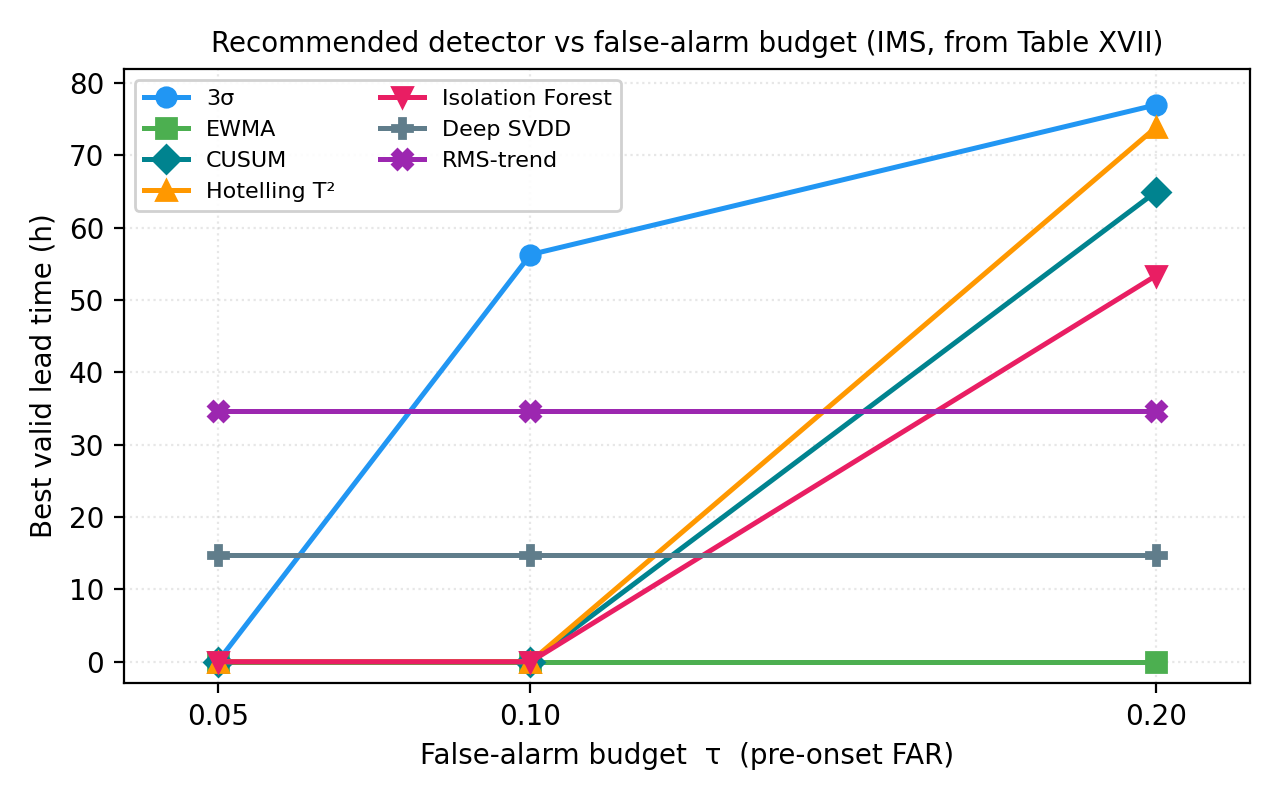
\includegraphics[width=0.94\columnwidth]{figs/fig_far_budget_detector.png}
\caption{Best \emph{valid} lead time per detector as a function of the false-alarm
budget $\tau$ on IMS, plotted directly from the operating points of
Table~\ref{tab:farsens}. Each line is one detector; a value of $0$ means no
operating point within budget. The recommended detector changes with $\tau$:
3$\sigma$ wins at $\tau\ge0.10$, while at a strict $\tau{=}0.05$ only the low-FAR
Deep SVDD and the RMS-trend floor remain valid.}
\label{fig:farbudget}
\end{figure}


\textbf{Where does $\tau{=}10\%$ come from? A cost-ratio argument.} We do not treat
$\tau$ as arbitrary. Consider a simple expected-cost model with two site parameters:
$c_I$, the cost of responding to one nuisance alarm (a wasted inspection), and $c_F$,
the cost of an unplanned bearing failure (downtime plus secondary shaft/housing damage).
Over a bearing's pre-onset life of $k$ windows a detector at pre-onset FAR $f$ issues
$\approx k f$ nuisance inspections, and a valid alarm with adequate lead converts the
failure into a planned repair, saving $c_F$. An operator should tolerate false alarms up
to the budget at which their cumulative cost equals the warning's value,
$k\,\tau\,c_I \approx c_F$, i.e.
\begin{equation}
\tau^{\ast} \approx \frac{c_F}{k\,c_I} = \frac{\rho}{k}, \qquad \rho \equiv c_F/c_I .
\label{eq:taustar}
\end{equation}
For rolling-element bearings an unplanned failure typically costs $\rho{=}10^2$--$10^4$
times a routine inspection, and the pre-onset window count is of order $k{\sim}10^3$ on
the runs studied here, so \eqref{eq:taustar} places the break-even budget at
$\tau^{\ast}\!\sim\!0.1$--$1$ (Table~\ref{tab:taustar_grid}): our $\tau{=}0.10$ is the
\emph{conservative} end of that range and is justified whenever failures are at least $\sim$100$\times$ costlier than
inspections. The strict $\tau{=}0.05$ column of Table~\ref{tab:farsens} corresponds to
the opposite regime---inspections that are themselves disruptive (e.g.\ requiring a
shutdown), so $\rho$ is small---exactly where the low-FAR Deep SVDD point becomes the
economical choice. We stress this is an \emph{order-of-magnitude} anchor, not a
site-specific optimisation: the true optimum requires an operator's actual $c_I$ and
$c_F$, which we do not have, and Eq.~\eqref{eq:taustar} is offered so a practitioner can
substitute their own.

\begin{table}[t]
\caption{The break-even budget $\tau^{\ast}=\rho/k$ from Eq.~\eqref{eq:taustar}
(clipped to $[0,1]$), over failure-to-inspection cost ratios
$\rho\in\{10^2,10^3,10^4\}$ and pre-onset window counts $k\in\{10^2,10^3,10^4\}$.
The chosen $\tau{=}0.10$ sits inside this range across the mid-to-high cost ratios
typical of rolling-element bearings, which is why it is a conservative central
choice. Every entry is computed directly from Eq.~\eqref{eq:taustar}; no
experimental quantity enters.}
\label{tab:taustar_grid}
\centering
\footnotesize
\setlength{\tabcolsep}{8pt}
\begin{tabular}{@{}lccc@{}}
\toprule
 & $\rho{=}10^2$ & $\rho{=}10^3$ & $\rho{=}10^4$ \\
\midrule
$k{=}10^2$ & 1.00 & 1.00 & 1.00 \\
$k{=}10^3$ & 0.10 & 1.00 & 1.00 \\
$k{=}10^4$ & 0.01 & 0.10 & 1.00 \\
\bottomrule
\end{tabular}
\end{table}


\begin{table}[t]
\caption{IMS lead-time--vs--false-alarm trade-off (mean across runs) at three
threshold percentiles. Up-and-to-the-left (high lead, low FAR) is better.
$\dagger$ marks operating points whose pre-onset FAR exceeds the
$\tau{=}10\%$ budget and are therefore \emph{invalid} under the gated metric---
their lead times are not usable warning times.}
\label{tab:tradeoff}
\centering
\footnotesize
\begin{tabular}{@{}lcccccc@{}}
\toprule
& \multicolumn{2}{c}{95th pct} & \multicolumn{2}{c}{99th pct}
& \multicolumn{2}{c}{99.5th pct} \\
\cmidrule(lr){2-3}\cmidrule(lr){4-5}\cmidrule(lr){6-7}
Method & Lead & FAR & Lead & FAR & Lead & FAR \\
\midrule
3$\sigma$        & 77.0 & 18.1$\dagger$ & 60.7 & 11.7$\dagger$ & 56.3 & \phantom{0}8.9 \\
EWMA             & 89.1 & 22.1$\dagger$ & 78.3 & 21.0$\dagger$ & 78.3 & 21.0$\dagger$ \\
CUSUM            & 65.0 & 19.4$\dagger$ & 64.2 & 19.0$\dagger$ & 64.2 & 19.0$\dagger$ \\
Hotelling $T^2$  & 176.9& 28.1$\dagger$ & 82.7 & 20.8$\dagger$ & 73.9 & 19.0$\dagger$ \\
Isolation Forest & 174.7& 27.1$\dagger$ & 75.8 & 20.6$\dagger$ & 53.4 & 19.8$\dagger$ \\
Deep SVDD        & 14.8 & \phantom{0}0.6 & \phantom{0}3.2 & 0.0 & \phantom{0}2.7 & 0.0 \\
RMS-trend        & 34.7 & \phantom{0}4.6 & \phantom{0}1.3 & 0.0 & 1.3 & 0.0 \\
\bottomrule
\end{tabular}
\end{table}

\begin{figure}[t]
\centering
\includegraphics[width=0.94\columnwidth]{figs/fig_tradeoff.png}
\caption{Lead-time vs pre-onset-FAR trade-off on IMS (threshold percentile
swept, mean across runs). Up-and-to-the-left is better. EWMA and Isolation
Forest dominate; the RMS-trend baseline collapses at low FAR.}
\label{fig:tradeoff}
\end{figure}

\begin{figure}[t]
\centering

\includegraphics[width=0.94\columnwidth]{figs/fig_tradeoff_xjtu.png}
\caption{Lead-time vs pre-onset-FAR trade-off on the ten XJTU-SY bearings
(threshold percentile swept, mean across bearings). The curve has the same
qualitative shape as IMS at the shorter absolute lead times XJTU's
short-lived bearings permit, showing the operating-point selection generalizes.}
\label{fig:tradeoff_xjtu}
\end{figure}

\subsection{Feature-group ablation}
Table~\ref{tab:ablation} ablates feature families on IMS for Isolation Forest,
reporting mean lead time, mean pre-onset FAR, and the valid-alarm fraction
across the three runs. The pattern is instructive and somewhat against
expectation. Spectral and envelope groups yield the \emph{longest raw} lead
times (99.4\,h for envelope) but the \emph{lowest validity}: they fire early in
part because they fire indiscriminately, accruing 23--29\% pre-onset FAR. The
\texttt{rms\_only} group, by contrast, yields the highest valid-alarm fraction
(1.00) at a near-zero pre-onset FAR (0.2\%), at the cost of a shorter raw lead.
In other words, once the false-alarm budget is enforced, the simple time-domain
amplitude statistics, not the elaborate frequency-domain features, carry the
usable prognostic signal on IMS.

To check that this recommendation is not specific to Isolation Forest, we repeat
the ablation for the four SPC charts and Deep SVDD (Table~\ref{tab:ablation_spc},
valid-alarm fraction by group). The conclusion holds across every non-sequence
detector: time-domain amplitude features (\texttt{rms\_only} or \texttt{time\_only})
give each detector its highest or tied-highest validity, and admitting spectral,
envelope, or the full feature set never improves validity for any of them. For the
memory-based control charts it \emph{sharpens}: \texttt{rms\_only} is the unique
group at which 3$\sigma$ and EWMA reach full validity (1.00 at $0\%$ pre-onset
FAR), and spectral/envelope/all collapse all four SPC charts (3$\sigma$, EWMA,
CUSUM, Hotelling $T^2$) to $0.33$ by driving their pre-onset FAR to $42$--$63\%$---
the variance-sensitive charts react violently to the noisy extra dimensions. Deep
SVDD is the instructive exception, and it fails for the \emph{opposite} reason:
its pre-onset FAR stays near $0\%$ under every feature set (it rarely
false-alarms), yet spectral features still cut its validity to $0.33$ (and to
$0.00$ for \texttt{spectral\_only}) by delaying or suppressing the alarm rather
than inflating the FAR---the frequency-domain dimensions hurt the one-class deep
model through missed detections, not false alarms. Either way the practical
recommendation is detector-general on IMS: under a false-alarm budget, restrict
every detector to time-domain amplitude features; frequency-domain features must
be admitted with care, most of all for the SPC charts.

\textbf{Robustness of the \texttt{rms\_only} recommendation to the logging rate.}
Because the recommendation is meant to guide SCADA deployments, we repeat the
feature-group ablation at every coarsening factor
(\texttt{src/feature\_coarsening\_ablation.py}; mean valid-alarm fraction over the
three IMS runs and the three ablation detectors 3$\sigma$/EWMA/Isolation Forest,
Table~\ref{tab:coarsen}). At native and $2\times$ resolution \texttt{rms\_only} is the
uniquely best group (valid fraction $1.00$), matching the full-resolution ablation
(Table~\ref{tab:ablation_spc}) and the informational argument that bin-averaging
preserves the amplitude statistic---the mean of a bin-averaged signal's RMS tracks
the RMS of the original, so \texttt{rms\_only} carries essentially the same signal
after aggregation. This validation holds cleanly at native and $2\times$ resolution
($f{=}1, 2$), where \texttt{rms\_only} is uniquely best and each IMS run contributes
enough windows to distinguish feature groups. At $f\ge5$ only a handful of windows
survive per run, so valid-alarm fractions move in steps of $1/3$ and the ranking
reflects few-window noise rather than stable feature-group differences---at $f{=}20$,
for instance, \texttt{time\_only} recovers to $0.89$ while \texttt{rms\_only} sits at
$0.67$, but this reversal rests on single-window differences per run and cannot be read
as a stable recommendation. The defensible reading is therefore: \texttt{rms\_only} is
the safest feature set at logging rates that retain enough windows to decide
($f\le2$), and no feature group displaces it at native resolution---consistent with the
non-destruction headline and the informational argument that bin-averaging preserves
the amplitude statistic exactly. Whether the \texttt{rms\_only} advantage holds at the
coarsest SCADA rates is not resolvable at $n{=}3$ and is left as an open empirical
question.

\begin{table}[t]
\caption{Feature-group valid-alarm fraction by coarsening factor on IMS
(3$\sigma$, EWMA, Isolation Forest; mean over the three runs \emph{and} the three
detectors), from the controlled coarsening ablation. \texttt{rms\_only} is uniquely
best at native and near-native resolution ($f{\le}2$); at $f\ge5$ the surviving-window
count is small and the fractions are coarse ($1/3$ steps), so the coarse-factor
columns read as directional rather than a stable ranking.}
\label{tab:coarsen}
\centering
\footnotesize
\setlength{\tabcolsep}{6pt}
\begin{tabular}{@{}lccccc@{}}
\toprule
Feature group & $f{=}1$ & $f{=}2$ & $f{=}5$ & $f{=}10$ & $f{=}20$ \\
\midrule
\texttt{rms\_only}      & \textbf{1.00} & \textbf{1.00} & 0.56 & 0.44 & 0.67 \\
\texttt{time\_only}     & 0.67 & 0.67 & 0.78 & 0.56 & 0.89 \\
\texttt{spectral\_only} & 0.44 & 0.56 & 0.67 & 0.56 & 0.67 \\
\texttt{all}            & 0.44 & 0.56 & 0.67 & 0.56 & 0.67 \\
\bottomrule
\end{tabular}
\end{table}

\begin{table}[t]
\caption{IMS feature-group ablation (Isolation Forest): mean lead time,
pre-onset FAR, and valid-alarm fraction across the three runs. Validity, not raw
lead, is the operationally meaningful column.}
\label{tab:ablation}
\centering
\footnotesize
\begin{tabular}{@{}lcccc@{}}
\toprule
Feature group & $d$ & Lead (h) & FAR$_{\mathrm{pre}}$ (\%) & Valid frac. \\
\midrule
rms\_only        & \phantom{0}8 & 32.0 & \phantom{0}0.2 & \textbf{1.00} \\
kurt\_only       & \phantom{0}5 & 60.2 & 16.2 & 0.67 \\
time\_only       & 20 & 63.4 & 18.8 & 0.67 \\
spectral\_only   & 30 & 70.6 & 23.4 & 0.67 \\
envelope\_only   & 16 & 99.4 & 29.3 & 0.67 \\
time+spectral    & 50 & 70.9 & 20.6 & 0.67 \\
all              & 50 & 70.9 & 20.6 & 0.67 \\
\bottomrule
\end{tabular}
\end{table}

\begin{table}[t]
\caption{Feature-group ablation generalized beyond Isolation Forest: valid-alarm
fraction (mean over the three IMS runs) by group for the four SPC charts, Deep
SVDD, and Isolation Forest. Time-domain amplitude features are best for every
detector; for the SPC charts \texttt{rms\_only} is uniquely (3$\sigma$, EWMA) or
jointly best and spectral/envelope/all collapse them to $0.33$ as their pre-onset
FAR rises to $42$--$63\%$, whereas Deep SVDD instead loses validity through missed
detections at near-zero FAR.}
\label{tab:ablation_spc}
\centering
\footnotesize
\setlength{\tabcolsep}{4pt}
\begin{tabular}{@{}lcccccc@{}}
\toprule
Feature group & 3$\sigma$ & EWMA & CUSUM & Hot.\ $T^2$ & D.\ SVDD & Iso.\ For. \\
\midrule
rms\_only      & \textbf{1.00} & \textbf{1.00} & \textbf{0.67} & \textbf{0.67} & \textbf{0.67} & \textbf{1.00} \\
kurt\_only     & 0.67 & 0.67 & 0.33 & 0.67 & 0.33 & 0.67 \\
time\_only     & 0.67 & 0.67 & 0.67 & 0.67 & 0.33 & 0.67 \\
spectral\_only & 0.33 & 0.33 & 0.33 & 0.33 & 0.00 & 0.67 \\
envelope\_only & 0.33 & 0.33 & 0.33 & 0.33 & 0.33 & 0.67 \\
time+spectral  & 0.33 & 0.33 & 0.33 & 0.33 & 0.33 & 0.67 \\
all            & 0.33 & 0.33 & 0.33 & 0.33 & 0.33 & 0.67 \\
\bottomrule
\end{tabular}
\end{table}

\subsection{Spectral vs time-domain features, per run}
A dedicated time-vs-spectral comparison (Table~\ref{tab:spectral}) confirms the
ablation at the level of individual runs and alarms. Adding spectral features to
the time-domain set does not improve valid detection on IMS, and on test~2 it
actively harms the control charts: the 3$\sigma$, EWMA, and Hotelling detectors
jump to 100\% pre-onset FAR (invalid) when spectral features are included, while
the same detectors are valid with time-only features. Isolation Forest, which is
less sensitive to a few noisy dimensions, remains valid in both settings. The
first test is unwarnable for every configuration because of its near-failure
onset, consistent with Table~\ref{tab:onset} and the conformal result. The
practical lesson is that frequency-domain features must be admitted with care
under a false-alarm budget: their extra sensitivity cuts both ways.

\begin{table}[t]
\caption{IMS spectral ablation, per run and detector (all six non-sequence
detectors): valid alarm (\checkmark) or invalid ($\times$) under time-only vs
time+spectral features. Spectral features inflate pre-onset FAR for the control
charts---3$\sigma$, EWMA, CUSUM, Hotelling $T^2$---on test~2, flipping each from
valid to invalid; Isolation Forest is robust to the extra noisy dimensions and stays
valid. Deep SVDD is the opposite failure mode: it is invalid on test~2 under
\emph{both} feature sets (a missed detection at near-zero FAR, not FAR inflation),
consistent with Table~\ref{tab:ablation_spc}. Test~1 is unwarnable for every
configuration.}
\label{tab:spectral}
\centering
\footnotesize
\begin{tabular}{@{}llcc@{}}
\toprule
Run & Detector & time-only & time+spectral \\
\midrule
\multirow{6}{*}{1st\_test}
 & 3$\sigma$        & $\times$ & $\times$ \\
 & EWMA             & $\times$ & $\times$ \\
 & CUSUM            & $\times$ & $\times$ \\
 & Hotelling $T^2$  & $\times$ & $\times$ \\
 & Deep SVDD        & $\times$ & $\times$ \\
 & Isolation Forest & $\times$ & $\times$ \\
\midrule
\multirow{6}{*}{2nd\_test}
 & 3$\sigma$        & \checkmark & $\times$ \\
 & EWMA             & \checkmark & $\times$ \\
 & CUSUM            & \checkmark & $\times$ \\
 & Hotelling $T^2$  & \checkmark & $\times$ \\
 & Deep SVDD        & $\times$ & $\times$ \\
 & Isolation Forest & \checkmark & \checkmark \\
\midrule
\multirow{6}{*}{3rd\_test}
 & 3$\sigma$        & \checkmark & \checkmark \\
 & EWMA             & \checkmark & \checkmark \\
 & CUSUM            & \checkmark & \checkmark \\
 & Hotelling $T^2$  & \checkmark & \checkmark \\
 & Deep SVDD        & \checkmark & \checkmark \\
 & Isolation Forest & \checkmark & \checkmark \\
\bottomrule
\end{tabular}
\end{table}

\subsection{Comparison with the Saxena prognostic horizon}
\label{sec:saxena}
If the false-alarm gate is what separates a usable warning from a manufactured one,
then a metric \emph{without} that gate should reward detectors our metric rejects.
We test this against the most widely used ungated warning-time metric---the Saxena
\emph{prognostic horizon} (PH) \cite{saxena2008,saxena2010}---and show that on IMS it
makes a different, and operationally wrong, detector recommendation.

The PH is the interval between a detector's first alarm and failure,
$\mathrm{PH}=\max\!\big(0,(t_f-\mathrm{FAT})/3600\big)$ hours, with \emph{no}
false-alarm constraint. It is exactly our lead time $L$ \emph{before} the validity
gate \eqref{eq:valid} is applied; that one missing conjunct is decisive.

\textbf{PH is maximized by the latch-on detector.} A detector that alarms from the
first sample earns the entire record as prognostic horizon.
Table~\ref{tab:latchon} evaluates this constant-on detector on the three IMS runs:
its PH is the full run length ($164$--$1073$\,h), yet it floods the whole pre-onset
region ($\mathrm{FAR}_{\mathrm{pre}}\!\approx\!1$), so the gated metric scores it
\emph{invalid} on every run ($L{=}0$). The oracle that fires just after the true
onset $t_o^{+}$ is the mirror image---zero pre-onset false alarms and the maximum
achievable lead. Under PH the latch-on detector is the clear winner; under $L$ it is
correctly scored worthless.

\begin{table}[t]
\caption{Latch-on detector under the Saxena prognostic horizon vs.\ the gated
metric $L$, on the three IMS runs. A constant-on detector (fires at $t{=}0$) earns
the full run length as PH but floods the pre-onset region
($\mathrm{FAR}_{\mathrm{pre}}\!\approx\!1$), so it is scored \emph{invalid}
($L{=}0$) on every run. The oracle fires just after the true onset $t_o^{+}$: zero
pre-onset false alarms and the maximum achievable lead ($t_f-t_o$).}
\label{tab:latchon}
\centering
\footnotesize
\begin{tabular}{@{}llcccc@{}}
\toprule
Detector & Run & PH (h) & $\mathrm{FAR}_{\mathrm{pre}}$ & $L$ (h) & Valid? \\
\midrule
\multirow{3}{*}{Latch-on ($t{=}0$)}
 & 1st\_test & \phantom{0}827.6 & $\approx$1.00 & 0.0 & no \\
 & 2nd\_test & \phantom{0}163.8 & $\approx$1.00 & 0.0 & no \\
 & 3rd\_test & 1073.3 & $\approx$1.00 & 0.0 & no \\
\midrule
\multirow{3}{*}{Oracle ($t_o^{+}$)}
 & 1st\_test & \phantom{0}12.9 & 0.00 & 12.9 & yes \\
 & 2nd\_test & \phantom{0}62.5 & 0.00 & 62.5 & yes \\
 & 3rd\_test & \phantom{0}44.5 & 0.00 & 44.5 & yes \\
\bottomrule
\end{tabular}
\end{table}

\textbf{PH and $L$ disagree on the real ranking.} The latch-on case is a worst-case
existence proof; the more damaging point is that PH and $L$ disagree on
\emph{deployable} detectors evaluated at their own best operating points.
Table~\ref{tab:phrank} ranks the seven non-sequence detectors on IMS by their best
raw lead (PH) and by their best lead at an operating point within the $\tau{=}10\%$
budget ($L$), both read from the threshold sweep of Table~\ref{tab:tradeoff}. The two
rankings are nearly inverted at the top. The four detectors PH ranks
highest---Hotelling $T^2$ ($176.9$\,h), Isolation Forest ($174.7$\,h), EWMA
($89.1$\,h), and CUSUM ($65.0$\,h)---each have \emph{no} valid operating point under a
$10\%$ false-alarm budget, so their gated lead is $L{=}0$. The detector PH ranks only
\emph{fourth}, 3$\sigma$ ($77.0$\,h raw), is the one that actually clears the budget
($56.3$\,h of lead at $8.9\%$ pre-onset FAR) and is the correct recommendation; Deep
SVDD, ranked last of the seven by PH, rises to a valid $14.8$\,h. The three deep
reconstruction models (omitted from the sweep) would sit \emph{above} all of these by
PH---raw leads of $200$--$215$\,h (Table~\ref{tab:ims_ci})---while alarming through
$48$--$100\%$ of every pre-onset region, i.e.\ $L{=}0$: the most extreme illustration
that PH rewards precisely the detectors a false-alarm-budgeted operator must avoid.

\begin{table}[t]
\caption{Detector rankings on IMS: Saxena prognostic horizon (PH, ungated best raw
lead) vs.\ the gated metric $L$ (best lead at an operating point within the
$\tau{=}10\%$ budget), both read from the threshold sweep of
Table~\ref{tab:tradeoff}; $L{=}0$ when no swept operating point is valid. The
rankings invert at the top: the detectors PH ranks best have no valid operating
point, while 3$\sigma$---PH's fourth---is the deployable winner. $^{\ast}$RMS-trend
is valid only at the loosest ($95$th-pct) threshold and on one of three runs (valid
fraction $0.33$), collapsing to $1.3$\,h under any tightening, whereas 3$\sigma$'s
valid point holds on two of three runs.}
\label{tab:phrank}
\centering
\footnotesize
\setlength{\tabcolsep}{4pt}
\begin{tabular}{@{}lccccc@{}}
\toprule
Method & PH (h) & PH rank & $L$ (h) & $L$ rank & Valid @$\tau{=}10\%$? \\
\midrule
Hotelling $T^2$  & 176.9 & 1 & \phantom{0}0.0 & 4 & no \\
Isolation Forest & 174.7 & 2 & \phantom{0}0.0 & 4 & no \\
EWMA             & \phantom{0}89.1 & 3 & \phantom{0}0.0 & 4 & no \\
3$\sigma$        & \phantom{0}77.0 & 4 & 56.3 & 1 & \textbf{yes} \\
CUSUM            & \phantom{0}65.0 & 5 & \phantom{0}0.0 & 4 & no \\
RMS-trend        & \phantom{0}34.7 & 6 & 34.7 & 2 & yes$^{\ast}$ \\
Deep SVDD        & \phantom{0}14.8 & 7 & 14.8 & 3 & yes \\
\bottomrule
\end{tabular}
\end{table}

\textbf{Implication.} Any warning-time metric that does not gate on
$\mathrm{FAR}_{\mathrm{pre}}$ can be driven to its maximum by loosening the alarm
threshold---in the limit, the constant-on detector. Our metric closes this by
construction; the Saxena PH does not. The distinction is not theoretical: on IMS it
changes the recommended detector from the ones PH ranks first by raw lead (Hotelling
$T^2$, Isolation Forest, EWMA) to 3$\sigma$, the only classical chart with a valid
operating point at a $10\%$ budget.

\subsection{Minimum training data for deep anomaly detectors}
\label{sec:mindata}
A practitioner commissioning condition monitoring at a new asset must decide how much
normal run-in history to collect before a deep model can be trusted over a simple
control chart. We quantify this on FEMTO---the one dataset where all six bearings are
long enough for every detector, including the seq-len-30 deep models, to run on the
full $n{=}6$---by sweeping the training fraction $T\in\{0.20,\dots,0.60\}$ (calibration
fixed at $0.10$, test $=1-T-0.10$) under the fixed Table~\ref{tab:hparams} protocol with
no per-$T$ retuning (\texttt{src/training\_sweep.py}). At no training fraction did any
bearing fail to form a length-30 sequence, so every cell is a genuine evaluation rather
than an N/A.

The result (Table~\ref{tab:trainsweep}, Fig.~\ref{fig:mindata}) is unambiguous and, we
think, more useful than a crossover point would have been: \emph{there is no
crossover}. The four magnitude control charts (3$\sigma$, EWMA, CUSUM, Isolation
Forest) reach their highest valid-alarm fraction ($0.67$--$0.83$ over the six bearings)
with as little as $T{=}0.20$ of run length and are stable or only mildly lower
thereafter. The three deep reconstruction models sit far below them at \emph{every}
training fraction (LSTM-AE and Transformer-AD $0.33$--$0.50$, TCN-AE $0.17$--$0.33$) and
do \emph{not} close the gap as $T$ grows---more commissioning data does not make them
competitive in this regime. Deep SVDD produces no valid alarm on any FEMTO bearing at
any $T$. The failure mode is the same as on IMS test~1 (Table~\ref{tab:tradeoff}):
Deep SVDD fires very late in the run---its threshold requires substantial
encoder-distance growth from the trained center before alarming---so on short FEMTO
bearings ($1.4$--$7.8$\,h) the first alarm arrives after or coincident with failure on
every bearing regardless of training fraction, giving $L{=}0$ uniformly. This is a
bearing-lifetime constraint, not a training-data constraint: the model is not
data-starved in the usual sense but structurally unable to alarm early enough on runs
this short. The valid fraction of the charts if anything edges \emph{down} slightly from
$T{=}0.20$ to $T{=}0.30$, an artifact of the shrinking test window on these short
($1.4$--$7.8$\,h) bearings rather than a data-hunger effect.

The practical recommendation is therefore sharper than ``collect more data'': for
short-lived assets like these bearings, SPC charts should be preferred
\emph{regardless} of how much run-in history is available, because the deep
reconstruction models do not overtake them anywhere in the $0.20$--$0.60$ training
range---consistent with their data-starved behavior on the short XJTU-SY bearings
(Section~\ref{sec:femto}). Whether a crossover appears on genuinely long-running
assets, where a deep model could see thousands rather than dozens of normal windows,
is the open question we flag in future work.

\begin{table*}[t]
\caption{Valid-alarm fraction vs.\ training fraction on FEMTO ($n{=}6$ bearings; fixed
Table~\ref{tab:hparams} protocol, no per-$T$ retuning). The SPC charts are stable and
best from $T{=}0.20$ onward; the deep reconstruction models (LSTM-AE, TCN-AE,
Transformer-AD) and Deep SVDD stay below them at \emph{every} training fraction and do
not close the gap as $T$ grows---\emph{there is no crossover} in the $0.20$--$0.60$
range on these short bearings. ``SPC mean'' is the mean over 3$\sigma$/EWMA/CUSUM/IF.}
\label{tab:trainsweep}
\centering
\footnotesize
\setlength{\tabcolsep}{5pt}
\begin{tabular}{@{}lccccccccc|c@{}}
\toprule
$T$ & 3$\sigma$ & EWMA & CUSUM & Hot.\ $T^2$ & IF & D.\ SVDD & LSTM-AE & TCN-AE & Tr-AD & SPC mean \\
\midrule
0.20 & 0.83 & 0.83 & 0.83 & 0.67 & 0.83 & 0.00 & 0.50 & 0.33 & 0.50 & \textbf{0.83} \\
0.30 & 0.83 & 0.67 & 0.67 & 0.50 & 0.67 & 0.00 & 0.33 & 0.17 & 0.33 & 0.71 \\
0.40 & 0.83 & 0.67 & 0.67 & 0.50 & 0.67 & 0.00 & 0.33 & 0.17 & 0.33 & 0.71 \\
0.50 & 0.67 & 0.67 & 0.67 & 0.50 & 0.67 & 0.00 & 0.33 & 0.17 & 0.33 & 0.67 \\
0.60 & 0.67 & 0.67 & 0.67 & 0.50 & 0.67 & 0.00 & 0.33 & 0.17 & 0.33 & 0.67 \\
\bottomrule
\end{tabular}
\end{table*}

\begin{figure}[t]
\centering
\includegraphics[width=\columnwidth]{figs/fig_training_sweep.png}
\caption{Valid-alarm fraction vs.\ training fraction on FEMTO ($n{=}6$). SPC charts
(blue) sit at the top and are flat from $T{=}0.20$; the deep reconstruction models
(red) and Deep SVDD lie below the SPC baseline (dashed) at every training fraction and
never reach it---no crossover. More commissioning data does not make the deep models
competitive on these short bearings.}
\label{fig:mindata}
\end{figure}

\section{Discussion}

\subsection{What changed the story}
Four methodological corrections, applied together, change the conclusion of the
sampling study. First, a correct failure label for the third IMS test (which had
left a fifth of the data after the nominal failure) turns a guaranteed miss into
a valid detection. Second, an onset-gated metric that defeats the latch-on
exploit prevents a constant-on detector from manufacturing lead time. Third, a
$p<n$, channel-invariant feature space removes the ill-posedness of a
channel-count-dependent scheme. Fourth, a statistical test on the genuine unit
of inference---the run, not the within-run sampling factor---replaces an
eyeballed curve and a pseudoreplicated paired test. With all four in place, the
original claim that SCADA averaging destroys lead time is refuted on every
dataset tested, and the previously-reported significant positive effect is corrected
to a consistent but non-significant trend.

\subsection{Why the IMS trend appears but is neutral elsewhere}
The IMS trend has a clean candidate mechanism: bin-averaging is a low-pass
filter that removes single-window noise spikes, so the variance-sensitive
control charts (3$\sigma$, EWMA) cross and hold their thresholds earlier under
aggregation than under decimation, which keeps the spikes. This is consistent
with the trend concentrating in those detectors and being weakest for Isolation
Forest, which is robust to isolated spikes by design. The IMS trend is reproduced by an ordinary moving-average or Kalman filter on the
decimated stream (Appendix~D), indicating a generic low-pass-smoothing mechanism
rather than historian averaging specifically. On ONGC the data is already
smoothed at the 10\,s historian rate, so further aggregation adds little; on
XJTU the bearings are short-lived and many fail abruptly, so there is little
quiet runway over which averaging could help. The honest synthesis is therefore
not ``averaging helps'' but \emph{non-destruction}: across very different
regimes, coarse aggregation never costs warning time, and where the signal is
noisy and the runway long it shows a consistent tendency to stabilize the health
statistic.

\textbf{The single-asset turbine case study.} The one real historian record in
our study---an ONGC gas-turbine low-pressure-compressor bearing logged at a
10\,s SCADA rate and ending in a genuine operator shutdown---has every detector
alarm roughly $35$\,h ahead of the labeled failure, with an aggregate-vs-decimate
difference of at most about a minute for every detector. Because it is a single
asset ($n{=}1$) we draw \emph{no} inference from it and exclude it from the
inferential family; we report it in full as a case study in Appendix~E. It is
nonetheless the cleanest illustration of the practical question---it uses no
simulated coarsening---and is consistent with non-destruction.

\subsection{Practical implications}
For practitioners the message is reassuring and actionable. Storing
bin-averaged vibration at SCADA rates---the default behavior of most
historians---does not inherently sacrifice bearing-fault warning time relative
to keeping decimated raw samples, and may even improve it for control-chart
detectors on noisy long-runway data. The conformal results add a usable, distribution-free false-alarm
guarantee \emph{wherever the normal region is genuinely stationary}, and the
trade-off curve turns the gated metric into an operating-point selector for a
stated false-alarm budget. The ablations caution that more features are not
better under a false-alarm budget: time-domain amplitude and impulsiveness
statistics carry the usable signal on IMS, and spectral features must be
admitted with care.

Operators whose cost structure penalizes false alarms heavily---for instance,
process plants where each alarm triggers a mandatory manual inspection---have a
complementary operating point available. Deep SVDD consistently stays within budget
at $\le0.6\%$ pre-onset FAR across the swept threshold levels on IMS
(Table~\ref{tab:tradeoff}), achieving $14.8$\,h of advance warning with near-zero
false alarms. Where 3$\sigma$ maximizes warning time within the $10\%$ budget, Deep
SVDD minimizes nuisance alarms for operators requiring near-zero tolerance. Neither
should be used on IMS test~1, which the conformal machinery correctly flags as
uncalibrated (Table~\ref{tab:calib}).

\subsection{Summary of key outcomes}
In one place, the numbers that matter. \textbf{(1)~Non-destruction holds on all four inferential
datasets (and the single-asset case study):} SCADA bin-averaging never costs lead
time relative to decimation. \textbf{(2)~On IMS}, aggregation gives a positive but
\emph{non-significant} trend---same sign in all three runs for every magnitude
detector (3$\sigma$ \textbf{$+18.4$\,h} median, IF \textbf{$+12.2$\,h}, EWMA
\textbf{$+5.8$\,h}, CUSUM $+5.4$\,h, Hotelling $T^2$ $+4.6$\,h), but the exact
sign test floors at \textbf{$p{=}0.25$} at $n{=}3$. \textbf{(3)~Elsewhere the
effect is null:} the single-asset ONGC case study differs by \textbf{$\le1$\,min},
and XJTU-SY
($n{=}10$), FEMTO ($n{=}6$), and Ferrara ($n{=}6$) by \textbf{$\le8$\,min} median,
with Isolation Forest \emph{reversing sign} on FEMTO. \textbf{(4)~After Holm correction} across
the \textbf{$N{=}40$} detector\,$\times$\,dataset family, \textbf{no hypothesis
survives} (smallest adjusted $p{=}\mathbf{1.00}$). \textbf{(5)~Mechanism:} the
IMS advantage grows from $-0.35$\,h to \textbf{$+6.6$\,h} as SNR falls to 10\,dB
and is matched by a plain moving-average or Kalman filter on the decimated
stream---so the cause is \emph{generic low-pass smoothing}, not historian
averaging specifically. The honest, replicated headline is therefore
\textbf{non-destruction}, not ``aggregation helps.''

\section{Limitations and Threats to Validity}
\label{sec:threats}
We state the limits of the evidence plainly, grouped by the kind of validity
each concern bears on.

\textbf{External validity (generalization).} The IMS ``aggregation helps''
tendency is a sign-consistent but \emph{non-significant} trend ($n{=}3$;
Table~\ref{tab:ims_paired}) and does \emph{not} replicate on the larger XJTU
(Table~\ref{tab:xjtu_paired}) or FEMTO (Table~\ref{tab:femto_paired}) sets---on
FEMTO the only sign-consistent detector even trends in the \emph{opposite}
direction; we therefore claim only \emph{non-destruction} as
the cross-dataset headline, not a positive effect. ONGC is a single asset
($n{=}1$), reported as a descriptive case study with no inference
(Table~\ref{tab:ongc_paired}). The datasets, while deliberately diverse, are all rolling-element bearings; we do not claim the result transfers to
gearboxes, blades, or other failure modes without further testing.

\textbf{Residual gaming surfaces of the metric.} We claim the metric defeats the
specific latch-on (constant-on) exploit, not that it is unconditionally
ungameable, and we name two surfaces we do \emph{not} close. (a) A detector
could in principle align its alarm threshold to fire just after the onset time
$t_o^{+}$; because our onset is computed only from training-region statistics,
this cannot use test-region information, but an adversary with knowledge of the
onset rule could still tune toward it. (b) The onset health indicator shares its
RMS/kurtosis basis with several of the detectors' own features, so onset and
detection are not fully independent---a circularity that could, in principle,
favor detectors aligned to the onset statistic. We acknowledge both rather than
claim to have eliminated them; closing them (e.g.\ an onset signal disjoint from
the detector features) is future work.

\textbf{Construct validity (does the metric measure warning time?).} The onset
definition, although leakage-free and stable to its threshold multiplier across
$k\in\{3,4,5\}$ (Table~\ref{tab:onset}), is not the ground-truth
defect-initiation time, which is unobservable in these datasets. A late
onset---as on IMS test~1, where degradation and failure are nearly coincident
(Table~\ref{tab:onset})---inflates the pre-onset region, can mark a genuine
early detection invalid, and breaks the conformal exchangeability assumption
(Table~\ref{tab:calib}). The per-bearing XJTU breakdown
(Table~\ref{tab:xjtu_perbearing}) shows the same effect: bearings whose physics
provides essentially no warning runway score zero valid alarms regardless of
detector, which is correct behavior but means the valid-alarm fraction is partly
a property of the bearings, not only of the methods.

\textbf{Internal validity (is the comparison fair?).} We use a single fixed
hyperparameter protocol throughout to avoid optimistic per-condition tuning, and
we expose threshold sensitivity through the full trade-off sweep
(Fig.~\ref{fig:tradeoff}, Table~\ref{tab:tradeoff}) rather than reporting a
single hand-picked operating point. The controlled sampling sweep holds window
content and persistence constant so that the aggregate-vs-decimate contrast
isolates information loss; the few-windows regime at the largest coarsening
factor is annotated rather than hidden. Stochastic detectors inject their seed
explicitly so results are bit-reproducible.

\textbf{Statistical-conclusion validity.} Confidence intervals are wide on IMS
($n{=}3$); we resample runs, the genuine unit of generalization, rather than
seeds, which would understate uncertainty. Crucially, the five sampling factors
applied within a run are pseudoreplicates of one degradation trajectory, not
independent observations: an earlier pooled $15$-pair Wilcoxon test treated them
as independent and thereby overstated significance. We collapse to one
difference per run and apply an exact sign test, which at $n{=}3$ \emph{cannot}
fall below $p{=}0.25$; after Holm correction across the forty-test family
nothing is significant (Table~\ref{tab:holm}). The IMS result is therefore a
directional trend to be read together with the XJTU and FEMTO nulls, never as a
significant effect. A
parametric mixed-effects model is not used: with three random-effect levels it
would be over-fit, and the assumption-light sign test is the defensible choice
at this sample size. A formal power analysis makes the minimum-dataset requirement
concrete: to detect the observed IMS effect (Cohen's $d\approx0.7$--$1.2$ across the
magnitude detectors) at $\alpha{=}0.05$ and power $0.80$, a paired test needs
$n\approx6$ (at $d{=}1.2$) to $n\approx17$ (at $d{=}0.7$) independent run-to-failure
bearings; equivalently, the exact sign test we use cannot reach significance until at
least \emph{six} runs are sign-concordant ($2(\tfrac12)^6{=}0.031$). The three IMS runs
are thus a factor of two to five short of the sample size a significance claim would
require---the quantitative content of the ``long-runway, many-bearing campaign'' the
future work calls for. Confirming the IMS positive trend at statistical significance
requires a multi-bearing campaign with degradation windows measured in hours rather
than minutes. Long-runway bearing datasets with multiple runs are rare in the public
domain; the closest available single-bearing example is a KAIST bearing with a
$\sim$43-hour lifecycle ($n{=}1$, insufficient for inference). Research groups with
access to long-running industrial historian archives---gas turbines, compressors,
paper machines---can directly apply our released pipeline to test this hypothesis; we
provide loader templates for all public dataset formats used here to minimize
integration effort.

\section{Conclusion and Future Work}
We presented a lead-time-centric evaluation protocol for bearing anomaly
detection---one that defeats the latch-on exploit through an onset-gated,
false-alarm-budgeted metric---and used it to test whether SCADA-rate logging
destroys detection lead time. Across four inferential run-to-failure datasets---XJTU-SY ($n{=}10$),
FEMTO/PRONOSTIA ($n{=}6$), University of Ferrara ($n{=}6$), and NASA IMS
($n{=}3$)---together with a real single-asset turbine SCADA case study
(Appendix~E), coarse aggregation does not destroy lead time---and on IMS shows a consistent, sign-concordant positive
\emph{trend} for the variance-sensitive control charts (not statistically
significant at $n{=}3$, and not surviving multiple-comparison correction across
the $N{=}40$ family)---while
decimation is never better. The contribution is a reproducible methodology and
an honest, counter-intuitive empirical result: \emph{non-destruction}, not a
guaranteed positive effect. Future work will
learn the degradation onset jointly with the detector so that
the metric's anchor is independent of a hand-set health indicator (closing the
circularity noted in Section~\ref{sec:threats}), and extend the conformal
guarantee to the non-exchangeable early-degradation regime in which it currently
fails. A third direction concerns the minimum training-data requirement for deep
reconstruction models (Section~\ref{sec:mindata}), which we characterize here on
FEMTO bearings with $1.4$--$7.8$\,h lifetimes: verifying whether the crossover
training fraction generalizes to longer-running assets and different machinery types
is a natural extension. We release the full harness, detectors, tests, and the exact
tables and figures of this paper to support replication and extension
(Section~\ref{sec:availability}).

\section*{Appendix A: Reproducibility Settings}
Table~\ref{tab:hparams} lists the fixed hyperparameters used throughout, taken
verbatim from the released \texttt{config.py}. A single protocol is applied to
every detector, dataset, run, and sampling factor---no per-condition tuning.

\begin{table}[t]
\caption{Fixed hyperparameter protocol (from \texttt{config.py}). The onset
persistence/gap tolerances are in samples of the health-indicator series; at the
datasets' native intervals ($\sim$10\,min IMS, 1\,min XJTU, 10\,s FEMTO/ONGC) the
5/10-sample bars correspond to $\sim$50/100\,min, 5/10\,min, and 50/100\,s
respectively, so the tolerance is algorithmically---not physically---constant
across datasets. $^{\ast}$The pre-onset FAR is measured over the full pre-onset
window $t<t_o$ (Eq.~\ref{eq:valid}); a positional ``5\% of test'' parameter exists
in \texttt{config.py} for backward compatibility only and is used in no result
reported in this paper.}
\label{tab:hparams}
\centering
\footnotesize
\setlength{\tabcolsep}{4pt}
\begin{tabular}{@{}ll@{}}
\toprule
Setting & Value \\
\midrule
Feature window / overlap        & 10 samples / 50\% \\
Feature schema                  & channel-invariant, 49-dim \\
Train-fit feature cap           & top 50 (stratified) \\
Train / calibration / test      & 0.50 / 0.10 / 0.40 \\
Pre-onset FAR region            & full pre-onset window $t<t_o$ (Eq.~\ref{eq:valid})$^{\ast}$ \\
Onset health indicator          & rms\_kurt (amplitude/impulse) \\
Onset method / persistence      & terminal excursion / 5 samples \\
Onset $k\sigma$ / gap tolerance & $4\sigma$ / 10 samples \\
Alarm threshold / persistence   & 97.5th pct / 3 windows \\
FAR budget $\tau$               & 0.10 \\
Isolation Forest                & 200 trees, contam.\ auto \\
Hotelling $T^2$                 & PCA rank 10, $\alpha{=}0.01$ \\
EWMA / CUSUM                    & $\lambda{=}0.2,k{=}3$ / $k{=}0.5,h{=}5$ \\
Deep models (LSTM/TCN/Tr.)      & seq-len 30, 40--50 epochs, CPU \\
Transformer                     & $d_{\text{model}}{=}32$, 2 heads, 2 layers \\
FEMTO channels                  & horizontal + vertical accel.\ (both) \\
Conformal calibration fraction  & 0.10 \\
Bootstrap resamples             & runs, $B{=}2000$ \\
Random seed                     & 42 (into stochastic models) \\
Environment                     & Py 3.13, \texttt{requirements.lock.txt} \\
\bottomrule
\end{tabular}
\end{table}

\textbf{Computational cost.} Table~\ref{tab:cost} reports the wall-clock training
and per-window inference cost of each detector on the largest IMS run
($X_{\mathrm{train}}{=}631$, $X_{\mathrm{test}}{=}506$ windows, single CPU core,
median of five repeats). Training is a one-off offline step: the four SPC charts
and Hotelling $T^2$ fit in under 5\,ms, Isolation Forest and Deep SVDD in a
fraction of a second, and the three deep sequence models in $8$--$11$\,s. Inference
is negligible for every detector---at most $\sim$54\,$\mu$s per window (LSTM-AE),
five orders of magnitude below the fastest historian polling interval in our study
(10\,s, ONGC/FEMTO). Streaming condition monitoring at native SCADA rates is
therefore not compute-bound for any of the ten evaluated detectors, deep models included;
the only practical cost is the one-time CPU training of the sequence models.

\begin{table}[t]
\caption{Per-detector compute cost on the largest IMS run (631 train / 506 test
windows, single CPU core, median of five repeats). Training is one-off; inference
latency is per test window. Even the slowest model's inference is $\ll$ the 10\,s
SCADA polling interval.}
\label{tab:cost}
\centering
\footnotesize
\setlength{\tabcolsep}{5pt}
\begin{tabular}{@{}lrr@{}}
\toprule
Detector & Train (one-off) & Inference ($\mu$s/window) \\
\midrule
3$\sigma$          & $<1$\,ms          & $<0.1$ \\
EWMA               & $<1$\,ms          & $0.2$ \\
CUSUM              & $<1$\,ms          & $0.5$ \\
Hotelling $T^2$    & $4$\,ms           & $0.4$ \\
Isolation Forest   & $0.20$\,s         & $24$ \\
Deep SVDD          & $0.41$\,s         & $1.4$ \\
LSTM-AE            & $7.8$\,s          & $54$ \\
TCN-AE             & $10.5$\,s         & $47$ \\
Transformer-AD     & $10.3$\,s         & $38$ \\
\bottomrule
\end{tabular}
\end{table}

\section*{Appendix B: The 49-Dimensional Invariant Feature Space}
\label{app:features}
For full reproducibility we give the exact channel-invariant feature construction
(\texttt{src/features.py}, \texttt{extract\_invariant\_features}). Each snapshot's raw
waveform first yields six per-channel time-domain statistics
(Table~\ref{tab:featbase}). Each family is then made channel-count-invariant by
aggregating \emph{across} the physical channels with two operators---the channel
\emph{mean} and the channel \emph{max} (the worst-channel max is the classic
fault indicator)---and each aggregated series is summarised over the rolling window
(10 samples, $50\%$ overlap) by four descriptors: the window mean, standard deviation,
maximum, and least-squares linear-trend slope. This yields $6\times2\times4=48$
features; one cross-channel \emph{RMS-coherence} feature (the mean pairwise Pearson
correlation of the physical RMS channels within the window) brings the total to
\textbf{49}. Feature names follow the pattern
\texttt{\{family\}\_ch\{mean$|$max\}\_w\{mean$|$std$|$max$|$slope\}}, e.g.\
\texttt{rms\_chmax\_wslope} or \texttt{kurt\_chmean\_wmean}, plus the single
\texttt{rms\_coherence}. A train-fit variance top-$k$ selection ($k\le50$) then keeps
$p<n$; every statistic is fit on the training split only, so no test-region information
leaks into the features.

\begin{table}[h]
\caption{The six per-snapshot base statistics from which the 49-dim invariant space is
built. Each is computed per physical channel on the snapshot waveform $x$ (mean $\mu$,
std $\sigma$), then channel-aggregated (mean, max) and window-summarised (mean, std,
max, slope).}
\label{tab:featbase}
\centering
\footnotesize
\setlength{\tabcolsep}{5pt}
\begin{tabular}{@{}lll@{}}
\toprule
Statistic & Family & Per-snapshot formula \\
\midrule
RMS            & \texttt{rms}   & $\sqrt{\tfrac{1}{n}\sum_i x_i^2}$ \\
Kurtosis       & \texttt{kurt}  & $\tfrac{1}{n}\sum_i\!\big(\tfrac{x_i-\mu}{\sigma}\big)^4-3$ \\
Skewness       & \texttt{skew}  & $\tfrac{1}{n}\sum_i\!\big(\tfrac{x_i-\mu}{\sigma}\big)^3$ \\
Peak-to-peak   & \texttt{p2p}   & $\max_i x_i-\min_i x_i$ \\
Crest factor   & \texttt{crest} & $\max_i|x_i|\,/\,\mathrm{RMS}$ \\
Variance       & \texttt{var}   & $\tfrac{1}{n}\sum_i (x_i-\mu)^2$ \\
\midrule
\multicolumn{2}{@{}l}{Channel aggregations} & mean, max (over physical channels) \\
\multicolumn{2}{@{}l}{Window summaries}     & mean, std, max, slope \\
\multicolumn{2}{@{}l}{Cross-channel}        & \texttt{rms\_coherence} (1 feature) \\
\bottomrule
\end{tabular}
\end{table}

\section*{Appendix C: IMS Test-3 Relabeling Justification}
A subtlety we correct
here is the failure-label of the third test: an earlier label placed failure on
2004-04-08, leaving 21.5\% of the recorded data \emph{after} the nominal
``failure''---impossible for a run-to-failure series---so under that label the
third test is a guaranteed 100\% miss for every detector. We relabel it to the
last recorded sample (2004-04-18 02:42), at which the mean-RMS health indicator
has ramped from its flat baseline ($\sim$0.068) to $\sim$0.228 before the final
machine-off reading. We present this as an \emph{author relabeling based on the
health-indicator trajectory}, not an independently verified ground truth: we are not
aware of a published benchmark that corrects this label, so we do not claim it as a
community-established correction. It is nonetheless not a tuning choice: it only
affects the single hardest run, and it makes that run \emph{pass} rather than
improving any aggregate-vs-decimate contrast (the contrast is computed within each
run). It is the labeling we use throughout.

\section*{Appendix D: Mechanism --- Generic Smoothing vs Historian Averaging}
\label{sec:mechanism}
The IMS trend admits a clean candidate mechanism: bin-averaging is a low-pass
filter that suppresses single-window noise in the health statistic, letting the
alarm threshold be crossed earlier and held more persistently than under
decimation. If that is the mechanism, two predictions follow, and we test both
directly on IMS (\texttt{src/robustness.py}; controlling window content at
sampling factor~5 so only the smoothing differs).

\textbf{Prediction 1: the aggregate advantage should grow with noise.} We add
zero-mean Gaussian noise to the per-window health statistic at signal-to-noise
ratios of 30, 20, and 10\,dB and recompute the (aggregate~$-$~decimate) lead
time. To avoid the pseudoreplication we corrected in the main analysis, we
collapse the four magnitude-monitoring SPC charts---3$\sigma$, EWMA, CUSUM, and
Hotelling $T^2$ (Isolation Forest and Deep SVDD are excluded from the mechanism
tests as they are not single-statistic control charts on which a low-pass
argument acts directly)---to one mean difference \emph{per
run} and treat the run as the unit of inference ($n{=}3$ per level), rather than
pooling the four charts $\times$ three runs as twelve independent points. The
\emph{mean} advantage rises monotonically as noise increases
(Table~\ref{tab:noise}): from $-0.35$\,h at the native noise level to $+6.6$\,h
at 10\,dB, and at the two highest noise levels all three runs share the positive
sign. The lone large negative in the table, the $-7.94$\,h native-noise entry, is
IMS test~1---the abrupt near-coincident-onset run whose degradation begins only
$\sim$12\,h before failure (Table~\ref{tab:onset}), the same run that violates the
conformal guarantee (Table~\ref{tab:calib}) and is unwarnable in the spectral
ablation (Table~\ref{tab:spectral})---so its anomalous sign here is the same
internal-consistency story, not a new outlier. This is the qualitative signature of a low-pass mechanism---the noisier the
health signal, the more bin-averaging helps. We state its weight honestly: at
$n{=}3$ this is a \emph{directional} trend, not a significant effect (the exact
sign test floors at $p{=}0.25$, and at 30\,dB the per-run signs are mixed), the
same caveat that governs the main sweep. It corroborates the proposed mechanism;
it does not, and at this sample size cannot, establish it statistically.

\textbf{Prediction 2: any smoother on the decimated stream should recover the
advantage.} If the benefit is generic smoothing rather than the historian's
averaging specifically, then applying an ordinary smoother to the
\emph{decimated} stream should match bin-averaging. We compare a median filter,
a moving average, a constant-velocity Kalman filter, and a wavelet denoiser
against raw aggregation and raw decimation (Table~\ref{tab:denoise}). The moving
average and Kalman filter recover essentially the full aggregate lead time
($76.0$ and $75.7$\,h vs.\ aggregation's $75.7$\,h), while the median and wavelet
filters fall slightly short. The effect is therefore \emph{generic smoothing of
the health signal}, not a property unique to historian bin-averaging---an
operator who decimates and then lightly smooths recovers the same warning time.
This is an honest deflation of the ``aggregation helps'' framing: the practical
lesson is that the smoothing, not the storage policy, is what matters, and
non-destruction holds regardless.

Two entries in Table~\ref{tab:denoise} deserve a note. First, the linear
smoothers (moving average, Kalman) recover the advantage but the \emph{wavelet}
denoiser does not, dropping to $6/12$ valid alarms---below even raw decimation.
This is consistent with its being the one \emph{nonlinear} smoother in the set:
soft-thresholding of detail coefficients, with a universal threshold estimated
from the run's own noise floor, perturbs the pre-onset baseline (boundary and
shrinkage artifacts) enough to lift the pre-onset false-alarm rate past the budget.
The effect is measurable and localized: the two alarms lost relative to raw
decimation are both on test~2 (3$\sigma$ and Hotelling $T^2$), whose pre-onset FAR
rises from $0\%$ under raw decimation to $50\%$ under wavelet denoising---far past
the $10\%$ budget---while the gentle linear filters (median, moving average,
Kalman) leave that same baseline undisturbed and both charts valid. The lesson sharpens rather than breaks: smoothing that preserves the normal
baseline recovers the lead time, while smoothing that distorts it can cost
validity. Second, the validity counts at this sample size are themselves coarse---
raw decimation ($8/12$) edges aggregation ($7/12$) by a single alarm at
statistically indistinguishable lead times ($76.0$ vs.\ $75.7$\,h), so the
one-alarm gap is sampling noise at $n{=}12$, not evidence that decimation is
preferable; it is exactly the non-destruction headline restated. As in
Table~\ref{tab:noise}, we treat the run as the unit of inference and collapse the
four SPC charts to one mean difference per run ($n{=}3$); the valid-alarm counts at
this sample size are coarse and read as directional rather than precise.

\begin{table}[t]
\caption{IMS noise injection, \emph{run-level} (factor~5): the four
magnitude SPC charts (3$\sigma$, EWMA, CUSUM, Hotelling $T^2$) are collapsed to
one mean aggregate~$-$~decimate lead-time
difference per run, leaving the run as the unit of inference ($n{=}3$), exactly as
in Table~\ref{tab:ims_paired}. Per-run values are listed in the order (test~1,
test~2, test~3); the $-7.94$\,h native-noise entry is test~1, the abrupt
late-onset run. The mean advantage grows monotonically as SNR
falls---the signature of a low-pass mechanism---but at $n{=}3$ this is a
\emph{directional} trend that cannot be significance-tested (the exact sign test
floors at $p{=}0.25$), and at 30\,dB the per-run signs are in fact mixed.}
\label{tab:noise}
\centering
\footnotesize
\setlength{\tabcolsep}{4pt}
\begin{tabular}{@{}lcccc@{}}
\toprule
Noise (SNR) & Per-run agg$-$dec (h) [t1, t2, t3] & Mean (h) & Sign \\
\midrule
None (native) & $-7.94,\ +2.62,\ +4.28$ & $-0.35$ & $2/3$ \\
30\,dB        & $-0.44,\ -2.59,\ +5.95$ & $+0.97$ & $1/3$ \\
20\,dB        & $+10.60,\ +0.53,\ +0.12$ & $+3.75$ & $3/3$ \\
10\,dB        & $+14.99,\ +0.53,\ +4.28$ & $+6.60$ & $3/3$ \\
\bottomrule
\end{tabular}
\end{table}

\begin{table}[t]
\caption{IMS denoiser comparison (factor~5, four magnitude charts
3$\sigma$/EWMA/CUSUM/Hotelling $T^2$ collapsed to one mean per run,
$n{=}3$ runs, exactly as in Table~\ref{tab:noise}): mean lead time when a smoother
is applied to the \emph{decimated} stream, against raw aggregation and raw
decimation. A moving average or Kalman filter on the decimated stream recovers the
aggregate lead time, showing the benefit is generic smoothing rather than historian
averaging specifically. The validity column tallies the 12 chart$\times$run cells
and, at this sample size, is read as directional rather than precise.}
\label{tab:denoise}
\centering
\footnotesize
\begin{tabular}{@{}lcc@{}}
\toprule
Stream / denoiser & Mean lead (h) & Valid (of 12 cells) \\
\midrule
Aggregate (historian)        & $75.7$ & 7/12 \\
Decimate (raw)               & $76.0$ & 8/12 \\
Decimate + median            & $69.6$ & 8/12 \\
Decimate + moving average    & $76.0$ & 8/12 \\
Decimate + Kalman            & $75.7$ & 8/12 \\
Decimate + wavelet           & $73.2$ & 6/12 \\
\bottomrule
\end{tabular}
\end{table}

\section*{Appendix E: Supplementary --- Single-Asset Case Study (ONGC)}
\label{app:ongc}
\textbf{ONGC.} The ONGC record is a real Solar-Turbine low-pressure-compressor
(LPC) dataset: four vibration channels logged at a 10\,s SCADA rate over
$\sim$5 days (42{,}698 rows), ending in a genuine operator shutdown on
2023-11-13 09:46. This is authentic historian data with a real, documented
event---the maintenance record confirms the shutdown followed a rolling-element
bearing fault on the LPC---and the data-derived degradation onset
(2023-11-13 03:44) precedes the operator's action by roughly six hours. ONGC is
the only dataset that requires no simulated coarsening to be SCADA-rate: it is
the historian.

On genuine 10\,s industrial SCADA data ending in a real operator shutdown, every
detector achieves a long warning: 3$\sigma$, EWMA, Hotelling $T^2$, and
Isolation Forest each alarm roughly 35\,h before the labeled failure, and even
the naive RMS-trend baseline gives $\sim$22.8\,h. More to the point of this
paper, the aggregate-vs-decimate difference is at most about a minute for every
detector (Table~\ref{tab:ongc_paired}). Because ONGC is a \emph{single asset}
($n{=}1$), we treat it as a descriptive case study and draw \emph{no}
statistical inference from it---the differences below are reported as raw
magnitudes, not as a hypothesis test. On data that is already a real historian
stream, the choice of logging mechanism does not materially change warning time.
This is the cleanest possible illustration of the practical question---it uses
no simulated coarsening---and it is consistent with ``averaging is not the
enemy.''

\begin{table}[t]
\caption{ONGC real-turbine SCADA (single-asset case study, $n{=}1$; \emph{no
statistical inference}): descriptive aggregate $-$ decimate lead-time difference,
median over the five sampling factors. All differences are about a minute or less.}
\label{tab:ongc_paired}
\centering
\footnotesize
\begin{tabular}{@{}lc@{}}
\toprule
Method & Median $\Delta$ (min) \\
\midrule
3$\sigma$        & $+0.5$ \\
EWMA             & $-1.1$ \\
Hotelling $T^2$  & $+0.8$ \\
Isolation Forest & $+1.2$ \\
RMS-trend        & $\phantom{+}0.0$ \\
\bottomrule
\end{tabular}
\end{table}
\begin{figure}[t]
\centering
\includegraphics[width=0.86\columnwidth]{figs/fig_calibration_ongc.png}
\caption{Conformal calibration on the ONGC turbine ($n{=}1$ case study): empirical
pre-onset FAR vs target $\alpha$. The real historian stream tracks the diagonal
closely, a modest $1.5$--$2\times$ above target, consistent with a mostly-stationary
normal region.}
\label{fig:calib_ongc}
\end{figure}

\section*{Appendix F: Additional Detector --- Deep SVDD}
Deep SVDD~\cite{ruff2018} is evaluated alongside the nine headline detectors but
is not part of the headline set. It produced no valid alarm on any FEMTO bearing
at any training fraction (Table~\ref{tab:trainsweep}) and is omitted from the
headline count for that reason. Its numbers are retained, unchanged, throughout
the paper: the aggregate-vs-decimate results in
Tables~\ref{tab:ims_paired},~\ref{tab:xjtu_paired},~\ref{tab:femto_paired},
and~\ref{tab:ferrara_paired}; the $N{=}40$ Holm family in Table~\ref{tab:holm};
and its low-false-alarm operating point---$14.8$\,h of valid lead at $\le0.6\%$
pre-onset FAR---in Tables~\ref{tab:farsens},~\ref{tab:tradeoff},
and~\ref{tab:phrank}, where it is the recommended choice for operators with a
near-zero nuisance-alarm tolerance. We retain it in the statistical family
exactly as originally computed so that no $p$-value or family size changes.


\section*{Data and Code Availability}
\label{sec:availability}
All code---detectors, the leakage-free onset, the gated metric, the sampling
sweep, the conformal wrapper, the run-level statistical harness, and the
noise/denoiser mechanism test---is released with a pinned environment
(\texttt{requirements.lock.txt}, Python~3.13) and a test suite that asserts the
metric's resistance to the latch-on exploit, the leakage-free onset, and the
run-level sign-test/Holm machinery. Every table and figure in this paper is
generated directly from the released result files; no number is hand-edited.

\noindent\textbf{Repository:}
\url{https://github.com/Ansh-Goyal01/Scada-Leadtime-Benchmark}. A versioned
snapshot is archived on Zenodo at the concept DOI
\url{https://doi.org/10.5281/zenodo.20719076} (resolves to the latest version).

\noindent\textbf{Data.} The IMS (NASA), XJTU-SY, and FEMTO/PRONOSTIA
run-to-failure datasets are publicly available from their original providers; the
repository ships the loaders and the derived per-bearing feature caches needed to
reproduce every result. The ONGC gas-turbine SCADA record is proprietary and
covered by a non-disclosure agreement, so its raw \texttt{.xlsx} cannot be
redistributed; the derived health-indicator series and the figures/tables it
produces are included so the $n{=}1$ case study remains inspectable, and we note
that no headline statistical claim depends on it (ONGC is excluded from the
inferential family).

\begin{thebibliography}{00}
\bibitem{jardine2006} A. K. S. Jardine, D. Lin, and D. Banjevic, ``A review on machinery diagnostics and prognostics implementing condition-based maintenance,'' \emph{Mech. Syst. Signal Process.}, vol.~20, no.~7, pp.~1483--1510, 2006.
\bibitem{lee2014} J. Lee, F. Wu, W. Zhao, M. Ghaffari, L. Liao, and D. Siegel, ``Prognostics and health management design for rotary machinery systems---Reviews, methodology and applications,'' \emph{Mech. Syst. Signal Process.}, vol.~42, no.~1--2, pp.~314--334, 2014.
\bibitem{lei2018} Y. Lei, N. Li, L. Guo, N. Li, T. Yan, and J. Lin, ``Machinery health prognostics: A systematic review from data acquisition to RUL prediction,'' \emph{Mech. Syst. Signal Process.}, vol.~104, pp.~799--834, 2018.
\bibitem{si2011} X.-S. Si, W. Wang, C.-H. Hu, and D.-H. Zhou, ``Remaining useful life estimation---A review on the statistical data driven approaches,'' \emph{Eur. J. Oper. Res.}, vol.~213, no.~1, pp.~1--14, 2011.
\bibitem{saxena2008} A. Saxena, J. Celaya, E. Balaban, K. Goebel, B. Saha, S. Saha, and M. Schwabacher, ``Metrics for evaluating performance of prognostic techniques,'' in \emph{Proc. Int. Conf. Prognostics Health Manag. (PHM)}, 2008, pp.~1--17.
\bibitem{saxena2010} A. Saxena, J. Celaya, B. Saha, S. Saha, and K. Goebel, ``Metrics for offline evaluation of prognostic performance,'' \emph{Int. J. Prognostics Health Manag.}, vol.~1, no.~1, pp.~1--20, 2010.
\bibitem{goebel2011} K. Goebel, B. Saha, and A. Saxena, ``A comparison of three data-driven techniques for prognostics,'' in \emph{Proc. Machinery Failure Prevention Technol. (MFPT)}, 2011.
\bibitem{qiu2006} H. Qiu, J. Lee, J. Lin, and G. Yu, ``Wavelet filter-based weak signature detection method and its application on rolling element bearing prognostics,'' \emph{J. Sound Vib.}, vol.~289, no.~4--5, pp.~1066--1090, 2006.
\bibitem{wang2020} B. Wang, Y. Lei, N. Li, and N. Li, ``A hybrid prognostics approach for estimating remaining useful life of rolling element bearings,'' \emph{IEEE Trans. Rel.}, vol.~69, no.~1, pp.~401--412, 2020.
\bibitem{nectoux2012} P. Nectoux \emph{et al.}, ``PRONOSTIA: An experimental platform for bearings accelerated degradation tests,'' in \emph{Proc. IEEE Int. Conf. Prognostics Health Manag. (PHM)}, 2012, pp.~1--8.
\bibitem{arpa2024} L. Arpa, A. Gabrielli, M. Battarra \emph{et al.}, ``University of Ferrara run-to-failure vibration dataset of self-aligning double-row ball bearings,'' \emph{Data in Brief}, vol.~55, p.~110620, 2024, doi:10.1016/j.dib.2024.110620.
\bibitem{lessmeier2016} C. Lessmeier, J. K. Kimotho, D. Zimmer, and W. Sextro, ``Condition monitoring of bearing damage in electromechanical drive systems by using motor current signals of electric motors: A benchmark data set for data-driven classification,'' in \emph{Proc. European Conf. PHM Society}, 2016.
\bibitem{liu2008} F. T. Liu, K. M. Ting, and Z.-H. Zhou, ``Isolation forest,'' in \emph{Proc. IEEE Int. Conf. Data Mining (ICDM)}, 2008, pp.~413--422.
\bibitem{scholkopf2001} B. Sch\"olkopf, J. C. Platt, J. Shawe-Taylor, A. J. Smola, and R. C. Williamson, ``Estimating the support of a high-dimensional distribution,'' \emph{Neural Comput.}, vol.~13, no.~7, pp.~1443--1471, 2001.
\bibitem{vovk2005} V. Vovk, A. Gammerman, and G. Shafer, \emph{Algorithmic Learning in a Random World}. New York, NY, USA: Springer, 2005.
\bibitem{laxhammar2014} R. Laxhammar and G. Falkman, ``Online learning and sequential anomaly detection in trajectories,'' \emph{IEEE Trans. Pattern Anal. Mach. Intell.}, vol.~36, no.~6, pp.~1158--1173, 2014.
\bibitem{antoni2006} J. Antoni, ``The spectral kurtosis: A useful tool for characterising non-stationary signals,'' \emph{Mech. Syst. Signal Process.}, vol.~20, no.~2, pp.~282--307, 2006.
\bibitem{randall2011} R. B. Randall and J. Antoni, ``Rolling element bearing diagnostics---A tutorial,'' \emph{Mech. Syst. Signal Process.}, vol.~25, no.~2, pp.~485--520, 2011.
\bibitem{roberts1959} S. W. Roberts, ``Control chart tests based on geometric moving averages,'' \emph{Technometrics}, vol.~1, no.~3, pp.~239--250, 1959.
\bibitem{page1954} E. S. Page, ``Continuous inspection schemes,'' \emph{Biometrika}, vol.~41, no.~1--2, pp.~100--115, 1954.
\bibitem{hotelling1947} H. Hotelling, ``Multivariate quality control,'' in \emph{Techniques of Statistical Analysis}, C. Eisenhart \emph{et al.}, Eds. New York: McGraw-Hill, 1947.
\bibitem{montgomery2009} D. C. Montgomery, \emph{Introduction to Statistical Quality Control}, 6th ed. Hoboken, NJ, USA: Wiley, 2009.
\bibitem{hochreiter1997} S. Hochreiter and J. Schmidhuber, ``Long short-term memory,'' \emph{Neural Comput.}, vol.~9, no.~8, pp.~1735--1780, 1997.
\bibitem{malhotra2016} P. Malhotra, A. Ramakrishnan, G. Anand, L. Vig, P. Agarwal, and G. Shroff, ``LSTM-based encoder-decoder for multi-sensor anomaly detection,'' in \emph{Proc. ICML Anomaly Detection Workshop}, 2016.
\bibitem{hundman2018} K. Hundman, V. Constantinou, C. Laporte, I. Colwell, and T. Soderstrom, ``Detecting spacecraft anomalies using LSTMs and nonparametric dynamic thresholding,'' in \emph{Proc. ACM SIGKDD}, 2018, pp.~387--395.
\bibitem{ruff2018} L. Ruff \emph{et al.}, ``Deep one-class classification,'' in \emph{Proc. Int. Conf. Mach. Learn. (ICML)}, 2018, pp.~4393--4402.
\bibitem{vaswani2017} A. Vaswani \emph{et al.}, ``Attention is all you need,'' in \emph{Proc. Adv. Neural Inf. Process. Syst. (NeurIPS)}, 2017, pp.~5998--6008.
\bibitem{zhao2019} R. Zhao, R. Yan, Z. Chen, K. Mao, P. Wang, and R. X. Gao, ``Deep learning and its applications to machine health monitoring,'' \emph{Mech. Syst. Signal Process.}, vol.~115, pp.~213--237, 2019.
\bibitem{tautz2017} J. Tautz-Weinert and S. J. Watson, ``Using SCADA data for wind turbine condition monitoring---a review,'' \emph{IET Renew. Power Gener.}, vol.~11, no.~4, pp.~382--394, 2017.
\end{thebibliography}

\end{document}
